\section{Evaluation}
\label{sec:quantum_eval}

In this section, we evaluate our developed schemes.
We make two observations, which are as expected:  
(1) Performance of two-level methods is better than one-level methods in general, and 
(2) Performance of the PQC-based methods is superior to the QSD-based methods. 
In summary, our schemes are able to achieve meter-level (1-5m) localization accuracy, and near-perfect (99-100\%) classification accuracy in the case of discrete locations.

% (less than half a grid cell's dimensions) localization in a large area of $16\times16$ ($160m\times160m$), \pqcone achieves $6.2m$ of average localization error and \pqctwo achieves $4.7m$ of average localization error by using a network of 16 quantum sensors.}

\subsection{Evaluation Settings}

\para{Algorithms Evaluated.}
We evaluate four algorithms: \povmone, \povm, \pqcone, \pqctwo. As the name implies, \povmone and \pqcone are one-level methods, while \povm and \pqctwo are two-level methods.
Similarly, \povmone and \povm are QSD-based methods, while \pqcone and \pqctwo are PQC-based methods. We use the Regression Variant in our PQC-based methods by default, since in our default setting the transmitter can be anywhere in the 2D space.
%%%%%%
Our code\footnote{\url{https://github.com/caitaozhan/QuantumLocalization}} is written in Python and uses Numpy and Scipy libraries to perform matrix-related operations.
% which is the main part of the quantum sensing process and the QSD-based methods.

% We put more weight on evaluating the regression variation of the PQC-based methods since the continuous setting is closer to the real world.

\para{QSD-based Method Implementation.}
To implement the QSD-based methods, we first determine the target states which are then used to construct the pretty-good-measurement POVM via Eqn.~\ref{eqn:pgm}.
To localize a transmitter, we first compute the evolved state and then, use the POVM to determine the target state or the TX location. 
%%%%%%%%%%%%%%
This is done repeatedly as described in Section~\ref{sec:povm}, and in two levels (coarse, fine) depending on the localization scheme. 
The target states and evolved states are both generated using the sensor model described
in Section~\ref{sec:quantum_problem}, i.e., using Eqns.~\ref{eqn:unitary}-\ref{eqn:phase_shift}, with the electric field strength ($E$) and phase shift range modeled as below. 
% \magenta{Note that implementation of QSD-based methods does not require evaluating quantum circuits.}
% The sensor data is generated using the sensor model described in \S\ref{sec:problem}, i.e., using Eqns.~\ref{eqn:unitary}-\ref{eqn:phase_shift}, with the electric field strength ($E$) and phase shift range modeled as below. 
% \magenta{The hybrid circuits in PQC-based methods are implemented and trained in a separate quantum circuit simulator as described later. } 

\para{Generating Sensor Readings.}
The crux of determining target states, computing the evolved states, and simulating the training datasets is to compute the phase shift picked up by the quantum sensors due to the signal during the sensing process.
In Eqn.~\ref{eqn:phase_shift}, we modeled the phase shift as a function of the electric field strength and the sensing time.
Thus, we need a model for the electric field strength.
In free space, the electric field strength produced by a transmitter with an isotropic radiator can be approximated as~\cite{e-field-wiki}
$$E = \frac{\sqrt{30 \cdot P}}{d} \times (1 + noise) $$
where $E$ is the electric field strength in $V\cdot m^{-1}$, $P$ is the transmitter power output in $W$ (watt), and $d$ is the distance from the radiator in $m$.
Since in most quantum sensing applications, the signal to be sensed are weak signals, here we assume the power of the transmitter $P=0.1 \mu W$.
Ideally, the strength of the electric field is inverse to the distance between the transmitter and the sensor.
But in reality, the relationship is more complicated.
So, we add a random uniform variable $ noise\in[-0.05, 0.05]$ to incorporate reality in a simple way.
The target states and thus the POVMs are computed assuming zero noise during training, while during localization, the signal received is assumed to contain noise. 
The simulated datasets for PQC-based methods are assumed to contain noise too.

\softpara{Range of Phase Shift $\phi$.}
We set the sensing time $t'$ to 1 millisecond\footnote{In principle, the sensing time period must be smaller than the decoherence time, which varies across different quantum technologies.}. 
As mentioned later, our grid cells are $10m \times 10m$, and we assume 5 meters to be the minimum
distance allowed between a transmitter and a quantum sensor.
Thus, 
we choose 
the coupling constant $\gamma$ to be such that a quantum sensor at 5 meters away 
from the transmitter accumulates a phase shift of $2\pi$ during the sensing time $t'$; this entails
that the maximum phase shift is $2\pi$ and the minimum phase shift is as low as $0$ 
(when the sensor is very far away from the transmitter).

\para{PQC-Based Methods Implementation and Training.}
Different than the QSD-based methods, the PQC-Based methods involve quantum circuits.
We use the publicly available TorchQuantum~\cite{quantumnas2022} library to implement and train the parameterized hybrid circuits.
TorchQuantum's classes are inherited from a core class of PyTorch~\cite{pytorch}, which is used to implement the neural network predictor. 
% Thus, the training of the quantum part (PQC) and the classical part (neural network fully-connected layer) is seamlessly done together in PyTorch.
Thanks to PyTorch, we are able to train the PQCs fast on a GPU.
We use the Adam optimizer and train for 80 epochs for both \pqcone and \pqctwo methods.

The sensor readings are also used as the sensor data to train the PQC-based hybrid circuit models. 
Essentially, for a fixed initial global state of the sensors (say, $\psi$), each sample consists of the quantum state received from 
the quantum sensor network (input feature) and the location of the transmitter (ground truth target). 
More formally, each sample is of the kind: 
$(\bigotimes_{i=1}^{m} \hat{U}_i\ket{\psi}, L)$, where $\hat{U}_i$ is the evolution unitary operator for the $i^{th}$ quantum sensor (as per \S\ref{sec:quantum_problem} and above paragraphs), 
$\ket{\psi}$ is the uniform superposition initial state, and $L$ is the location of the transmitter in the field in all scenarios except for one, 
i.e., $L$ is the block number for samples used to train a ``coarse-level \pqcone'' in the \pqctwo Classifier Variant. 
We use one hundred training examples/samples for each cell, with the transmitter's location randomly scattered over the cell. 
%%%%%%%%%%%%%%%%%%%
For example, consider a $4\times4$ grid with a block length of 2.
The training dataset for \pqcone will have $16\times100=1600$ samples. 
And \pqctwo will have $16\times100=1600$ samples in the first level to train a ``coarse-level \pqcone'', and 
$4\times400=1600$ samples in the second level to train 4 blocks each requiring
$4\times100=400$ to train a ``fine-level \pqcone''.
Thus, there are a total of 3600 training samples used to train 5 models in a \pqctwo method.


\para{Quantum Sensor Deployment.} 
We deploy sensors uniformly over the area; for the \povm and  \pqctwo schemes, we deploy the fine-level sensors along the block borders so that the sensors can be used by the two neighbor blocks, i.e. fine-level sensors for the blocks are not disjoint.
%%%%%%%%%%%%%%%
We use a maximum of 8 quantum sensors for any single QSD instance---since the memory and computing requirements for storing and implementing a POVM become prohibitive beyond that. E.g., a POVM for 256 target-states over 12 sensors requires 69 GB of main memory storage.\footnote{We need $256$ matrices each of size $2^{12} \times 2^{12}$, with each matrix element being a complex number requiring 16 bytes.} 
%%%%%%%%%%%%%%%%%%%%%%%%%%%%%%%%%%
The PQC-based methods have a bottleneck on the number of sensors due to POVM considerations, but 
we are still limited in practice nevertheless due to training time and GPU memory; thus, we 
use a maximum of 16 sensors in the first level or in any block of the second level. This limits
the training time to at most several hours and GPU memory requirements to 8-16 GB. 
We discuss more details on number of sensors used at various levels and blocks, below.
Finally, each grid cell is of size $10m \times 10m$ in all settings, and the transmitter 
can be anywhere in the given area except that the minimum distance between any sensor
and transmitter is 5m.

\softpara{Two-Level Schemes: Blocks and Sensors Used.}
As described in \S\ref{sec:povm}, for a grid $N \times N$, if $N$ as a perfect square, 
the grid is divided into $\sqrt{N} \times \sqrt{N}$ blocks---with the first-level localizing the transmitter into one of the blocks, and the second-level localizing
the transmitter into a cell within the block.
%%%%%%%%%%%%
However, in this section, to get a better insight into the performance trends, in this section, we have also considered  $N$ values that are not perfect squares. 
%%%%%%%%%
For such $N$ values, we have determined block sizes as integers close to the $\sqrt{N}$; e.g., for a $12\times12$ grid, we divided the grid into $4 \times 4$ blocks each of $3 \times 3$ cells.
%%%%%%%%%%%%%%%%%
In terms of the number of sensors at each level---we use up to 16 sensors in the first-level of localization, but in the second-level we always use exactly 4 sensors per block irrespective of the block/grid size.

\para{Performance Metrics.} 
We use the {\tt Localization error} ($\lerr$, in meters) as the main metric to evaluate our localization schemes. $\lerr$ is defined as the distance between the actual location of the transmitter and the predicated location. 
In all plots except the CDF plots, average $\lerr$ refers to the
{\em average} localization error over many TX locations; 
in the CDF plots, the distribution is over many TX locations.

\subsection{Evaluation Results}
In our evaluation, we evaluate the performance of our proposed four localization algorithms' performances for varying  grid size and number of quantum sensors.
Note that, for one-level algorithms, the number of sensors is the total number of sensors used, while for the two-level algorithms, the number of sensors parameter is the number of sensors used in the first/coarse level (recall that, in the second level, we use only 4 sensors for each block). 
\begin{figure}[ht]
    \centering
    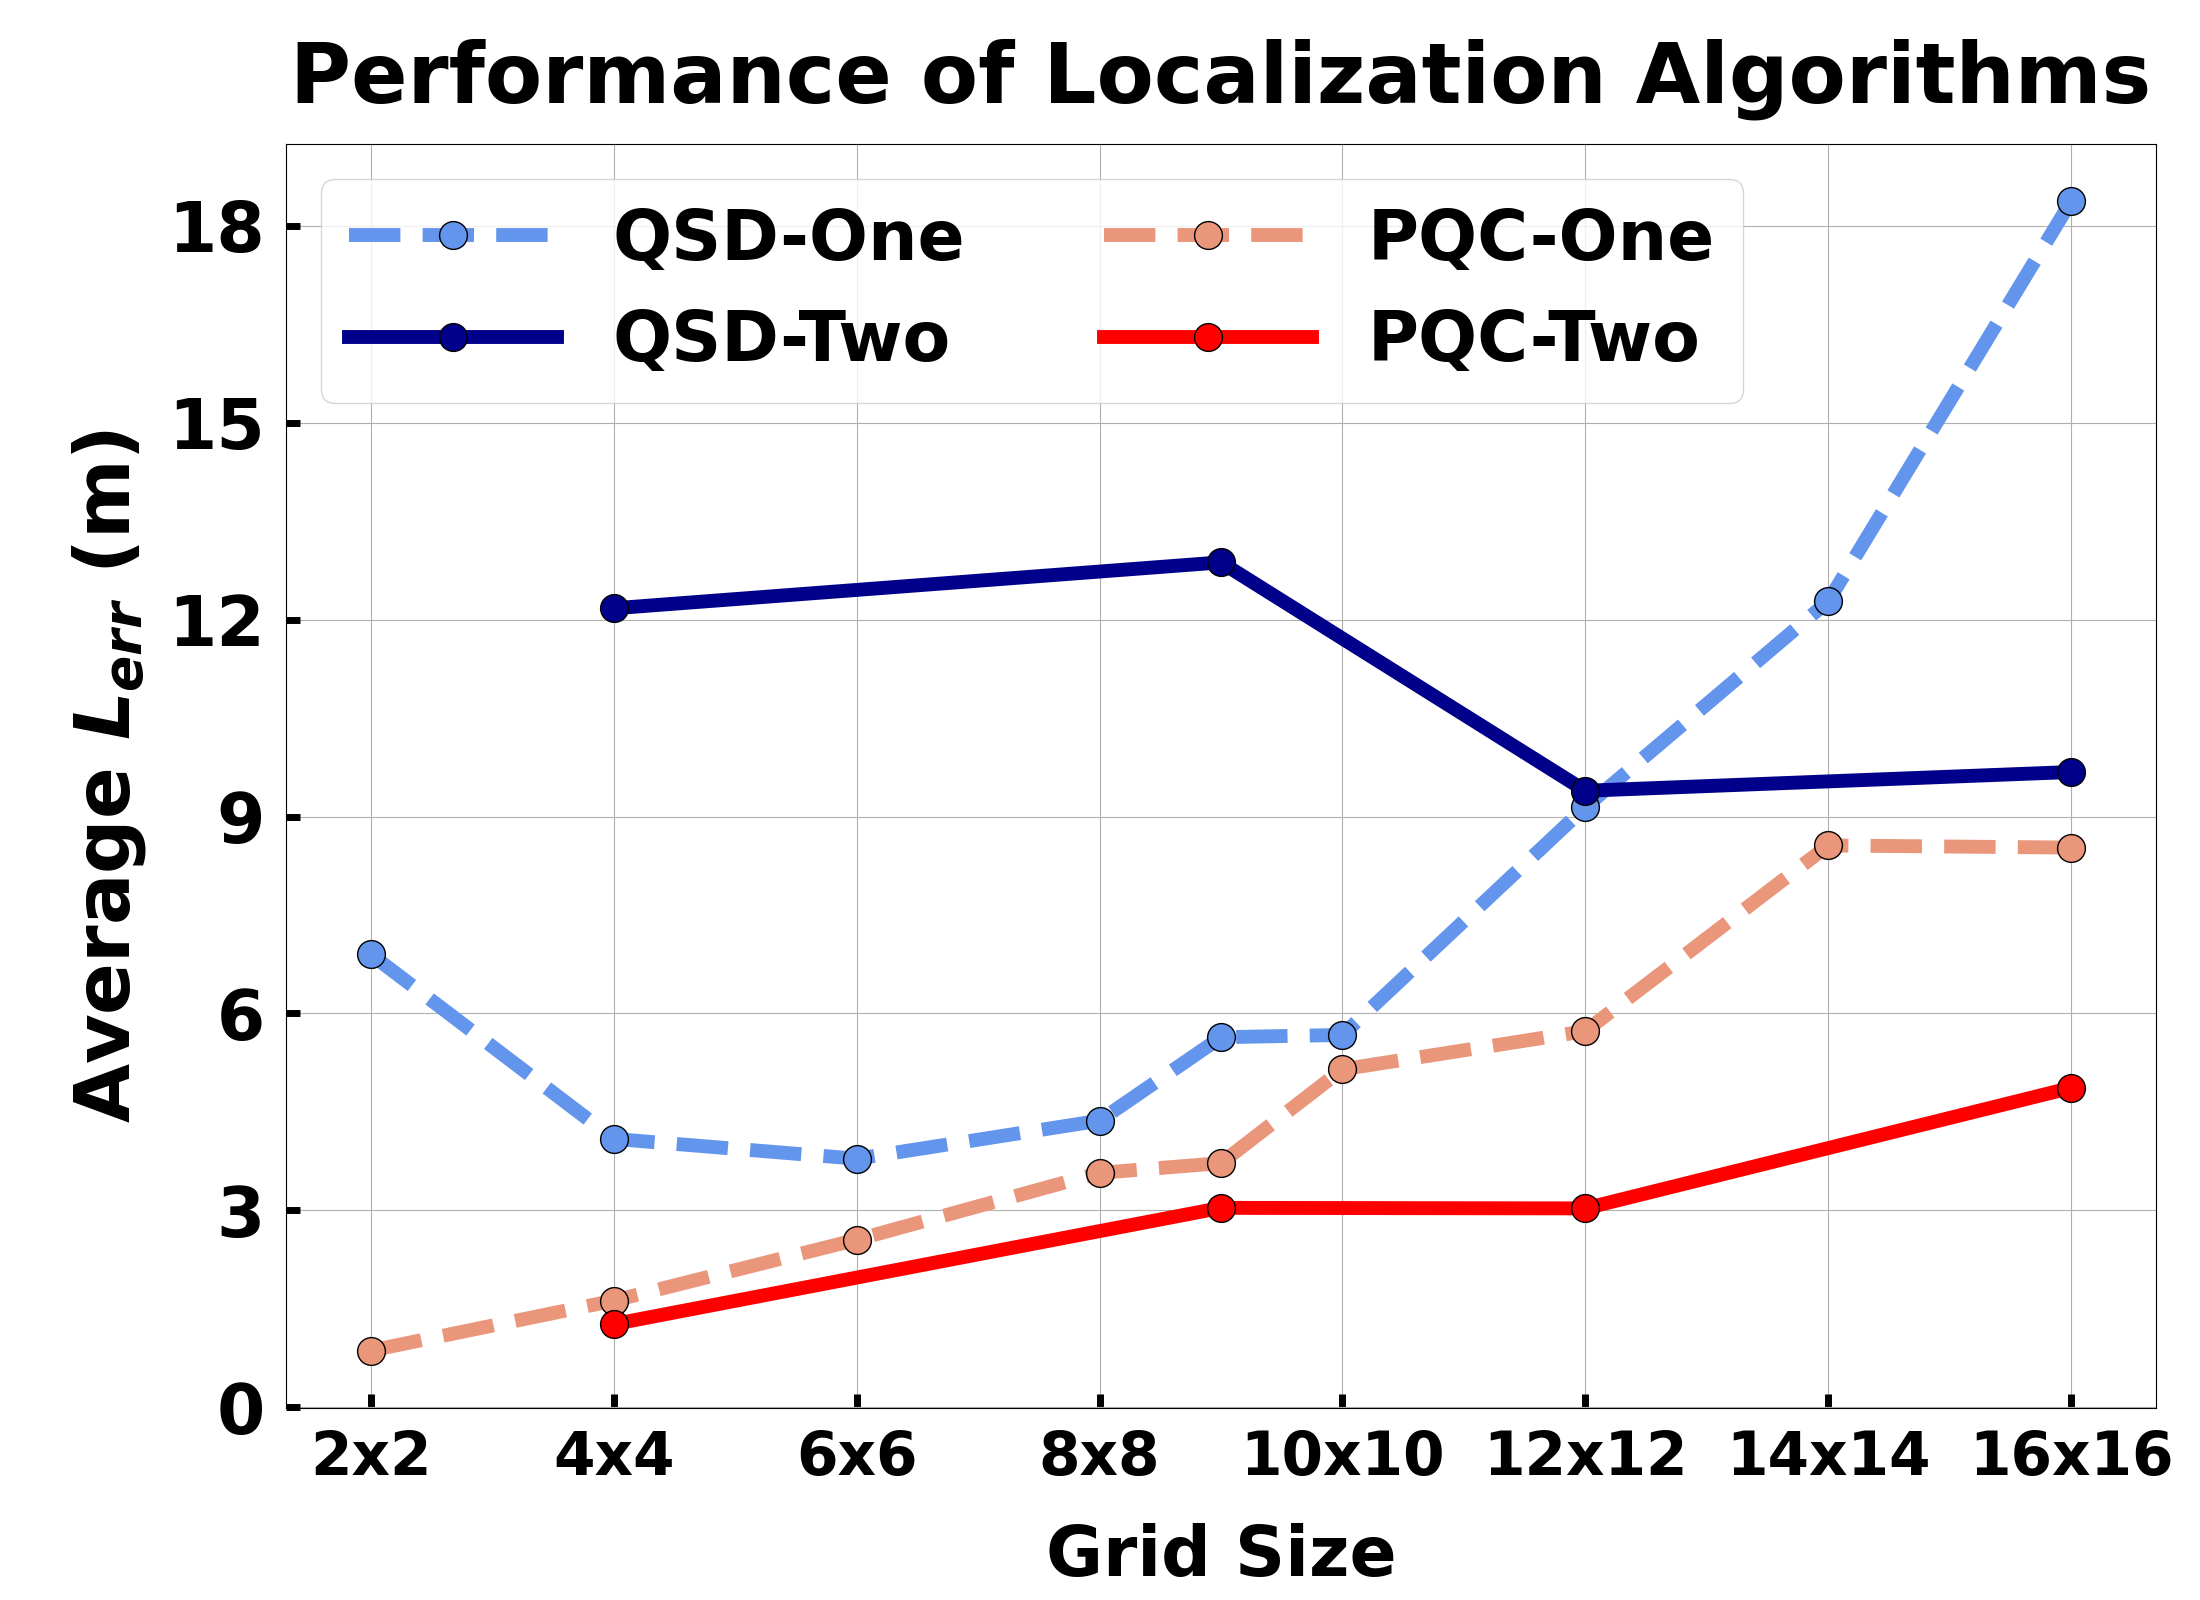
\includegraphics[width=0.8\textwidth]{chapters/qce/figures/continuous.varygrid.png}
    \caption{The performance of \povmone, \povm, \pqcone, \pqctwo for varying grid size and 8 quantum sensors.}
    \label{fig:continuous.varygrid}
\end{figure}

\para{Varying Grid Size.} Fig.~\ref{fig:continuous.varygrid} shows the performance of all four algorithms with varying grid sizes when the number of quantum sensors is eight. 
We observe that the PQC-based methods have lower localization error than the QSD-based methods, and
the two-level schemes generally perform better than one-schemes---except that the \povm performs worse than \povmone for smaller grid sizes.\footnote{This is likely because the QSD problem at the first/coarse level has a high error. 
The high error here is due to all cells being at the border edges, making the quantum state discrimination hard.
The neighboring two cells across the border of two blocks are close, thus hard to determine which block the cell is in.}
The results show the power of a well-trained parameterized hybrid circuit and the effectiveness of two-level schemes. 
More specifically, we observe that for a $16\times16$ grid, the average $\lerr$ of \pqctwo is $4.9 m$, which is almost half of the average $\lerr$ of \pqcone at $8.5m$.
Similarly, the $\lerr$ of \povm is also almost half of the $\lerr$ of \povmone, i.e., $9.6m$ vs $18.3m$.

\begin{figure}[ht]
    \centering
    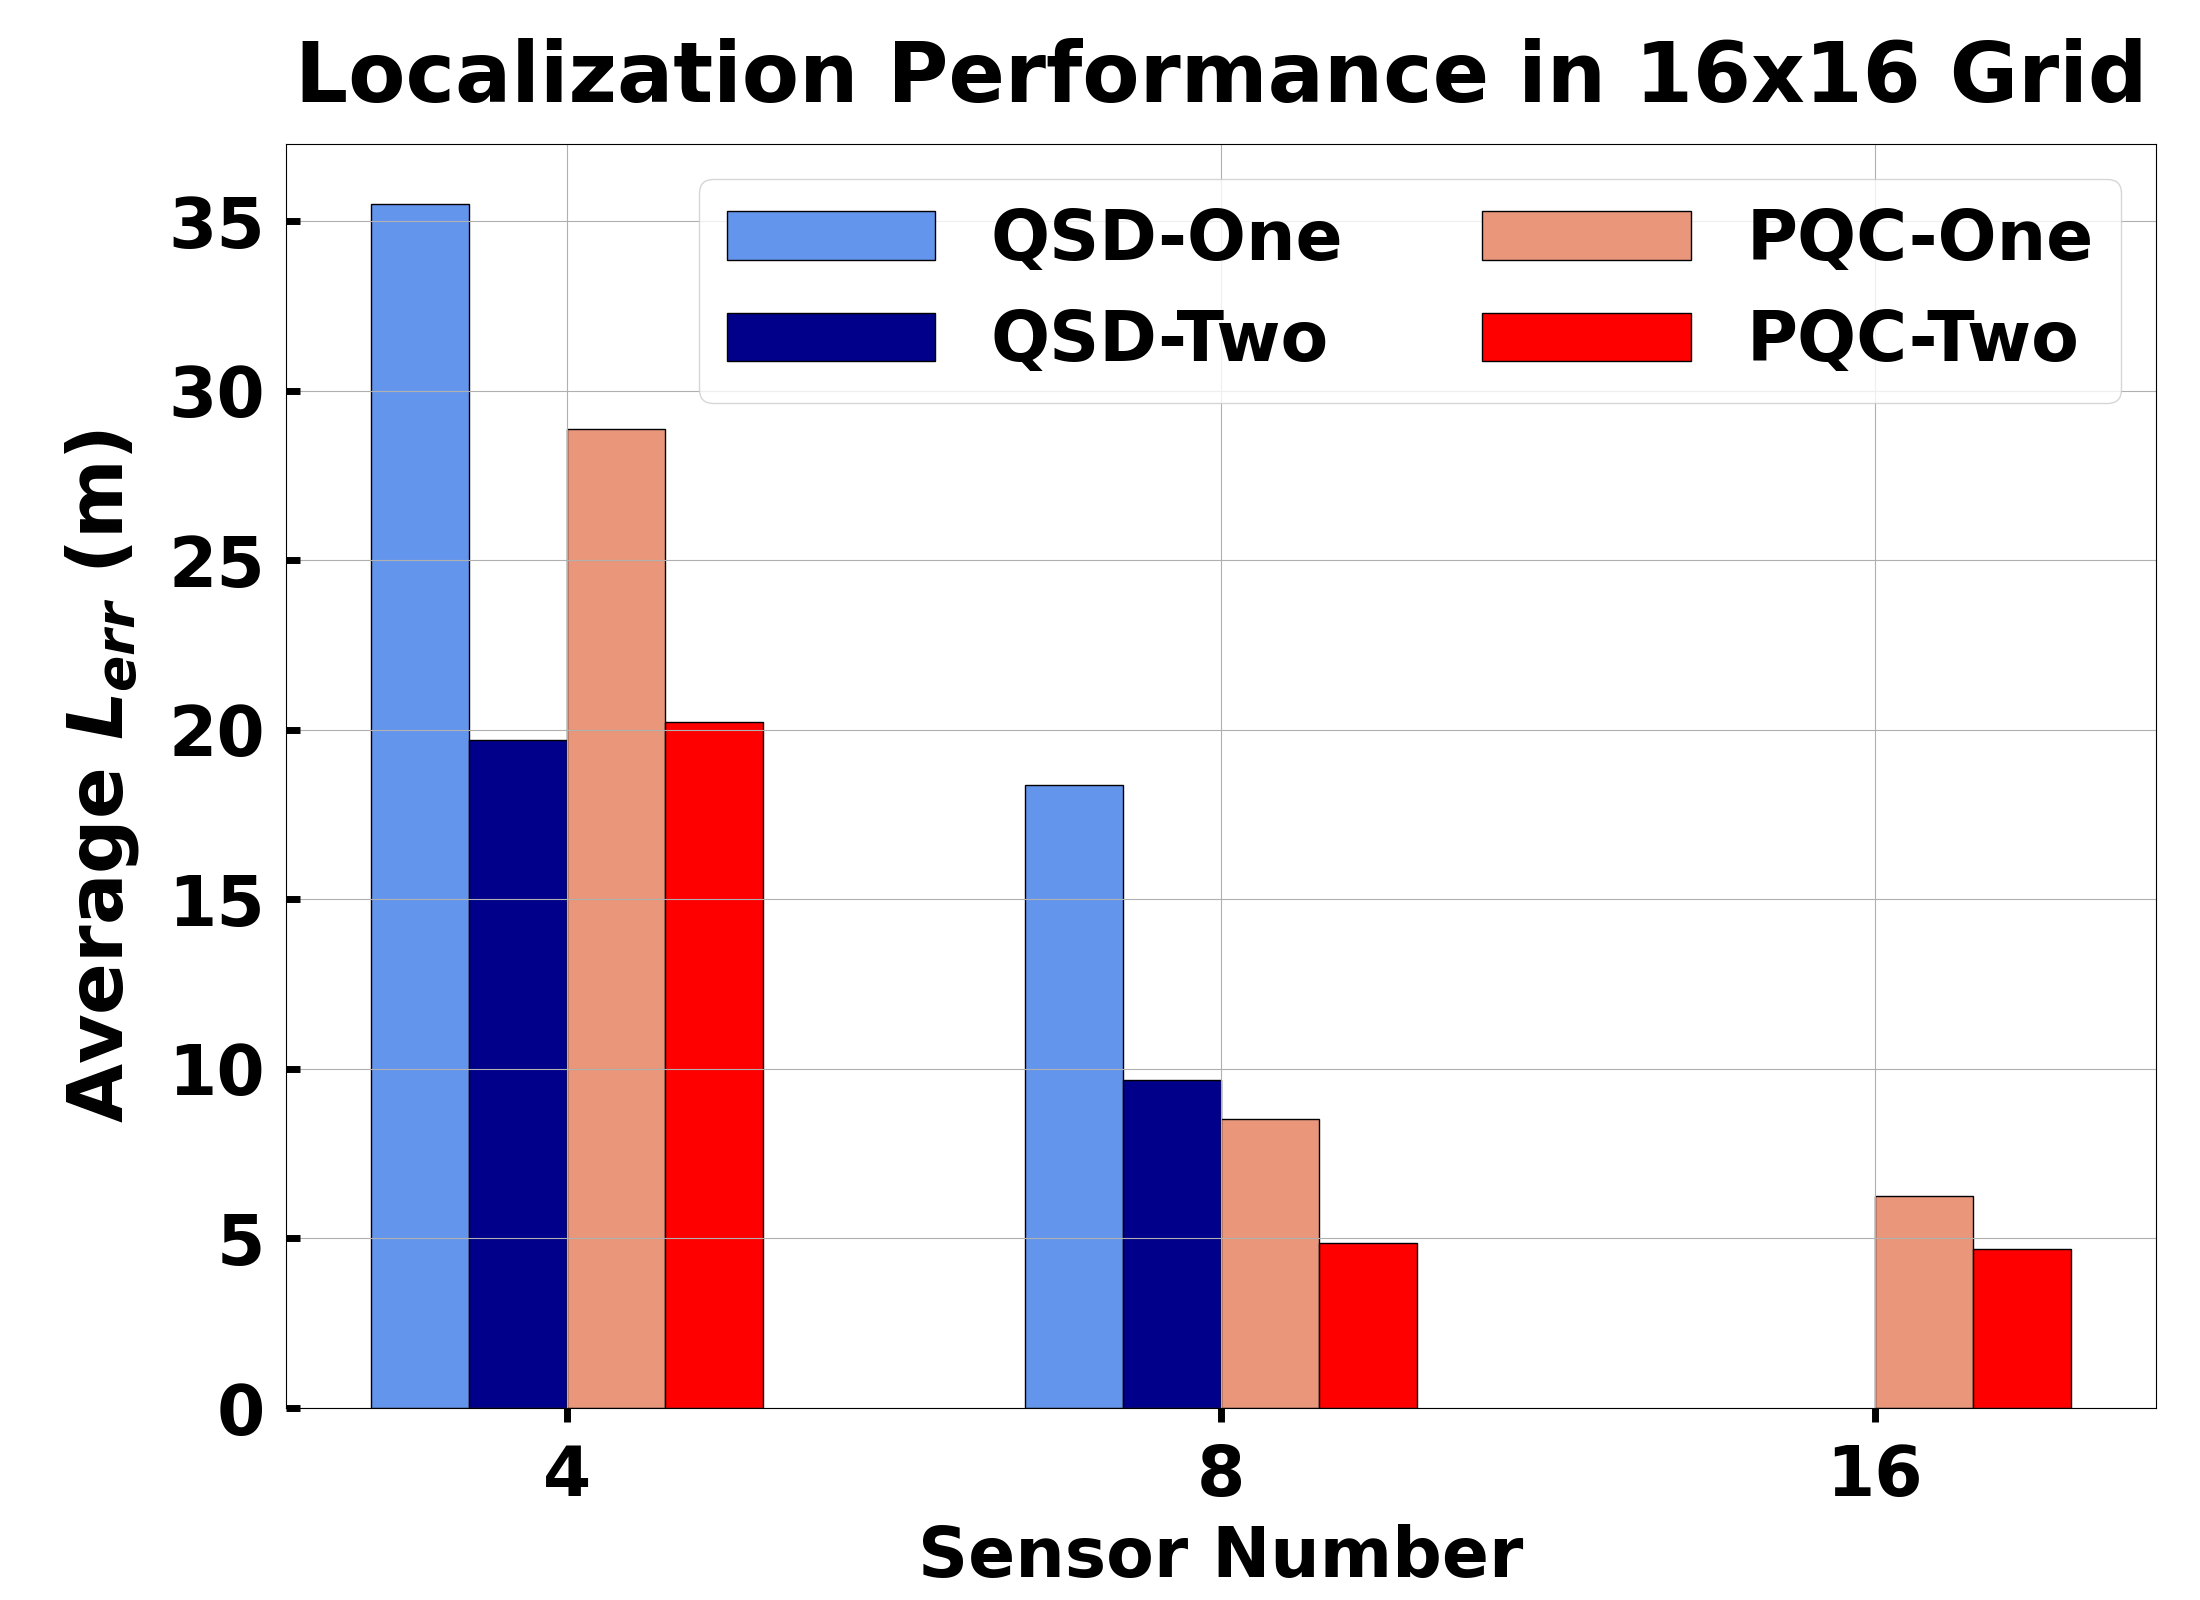
\includegraphics[width=0.8\textwidth]{chapters/qce/figures/continuous.varysensornum.png}
    \caption{The performance of \povmone, \povm, \pqcone, \pqctwo for varying sensor number and a $16\times16$ grid.}
    \label{fig:continuous.varysen}
\end{figure}

\para{Varying Number of Sensors.} 
Fig.~\ref{fig:continuous.varysen} shows the average $\lerr$ in a $16\times16$ grid with a varying number of quantum sensors.
As expected, we observe that the $\lerr$ improves with an increasing number of quantum sensors,
for all four schemes.
% This is because a larger number of quantum sensors is able to encode more information about the transmitter in a large grid, i.e., a higher number of quantum sensors can better cover the whole area.
For the \pqctwo scheme, we observe that the $\lerr$ improvement from 8 sensors to 16 sensors is minimal, i.e. $4.9 m$ vs $4.7 m$. 
This is because having 8 sensors in the first/coarse level seems sufficient to determine the block,
and then, in the second level, each block will always have 4 sensors associated with it (performance in the fine level is the same). 
% So there is no difference in the second level.
% So, the overall $\lerr$ difference for 8 sensors and 16 sensors is minimal.

\begin{figure}[ht]
    \centering
    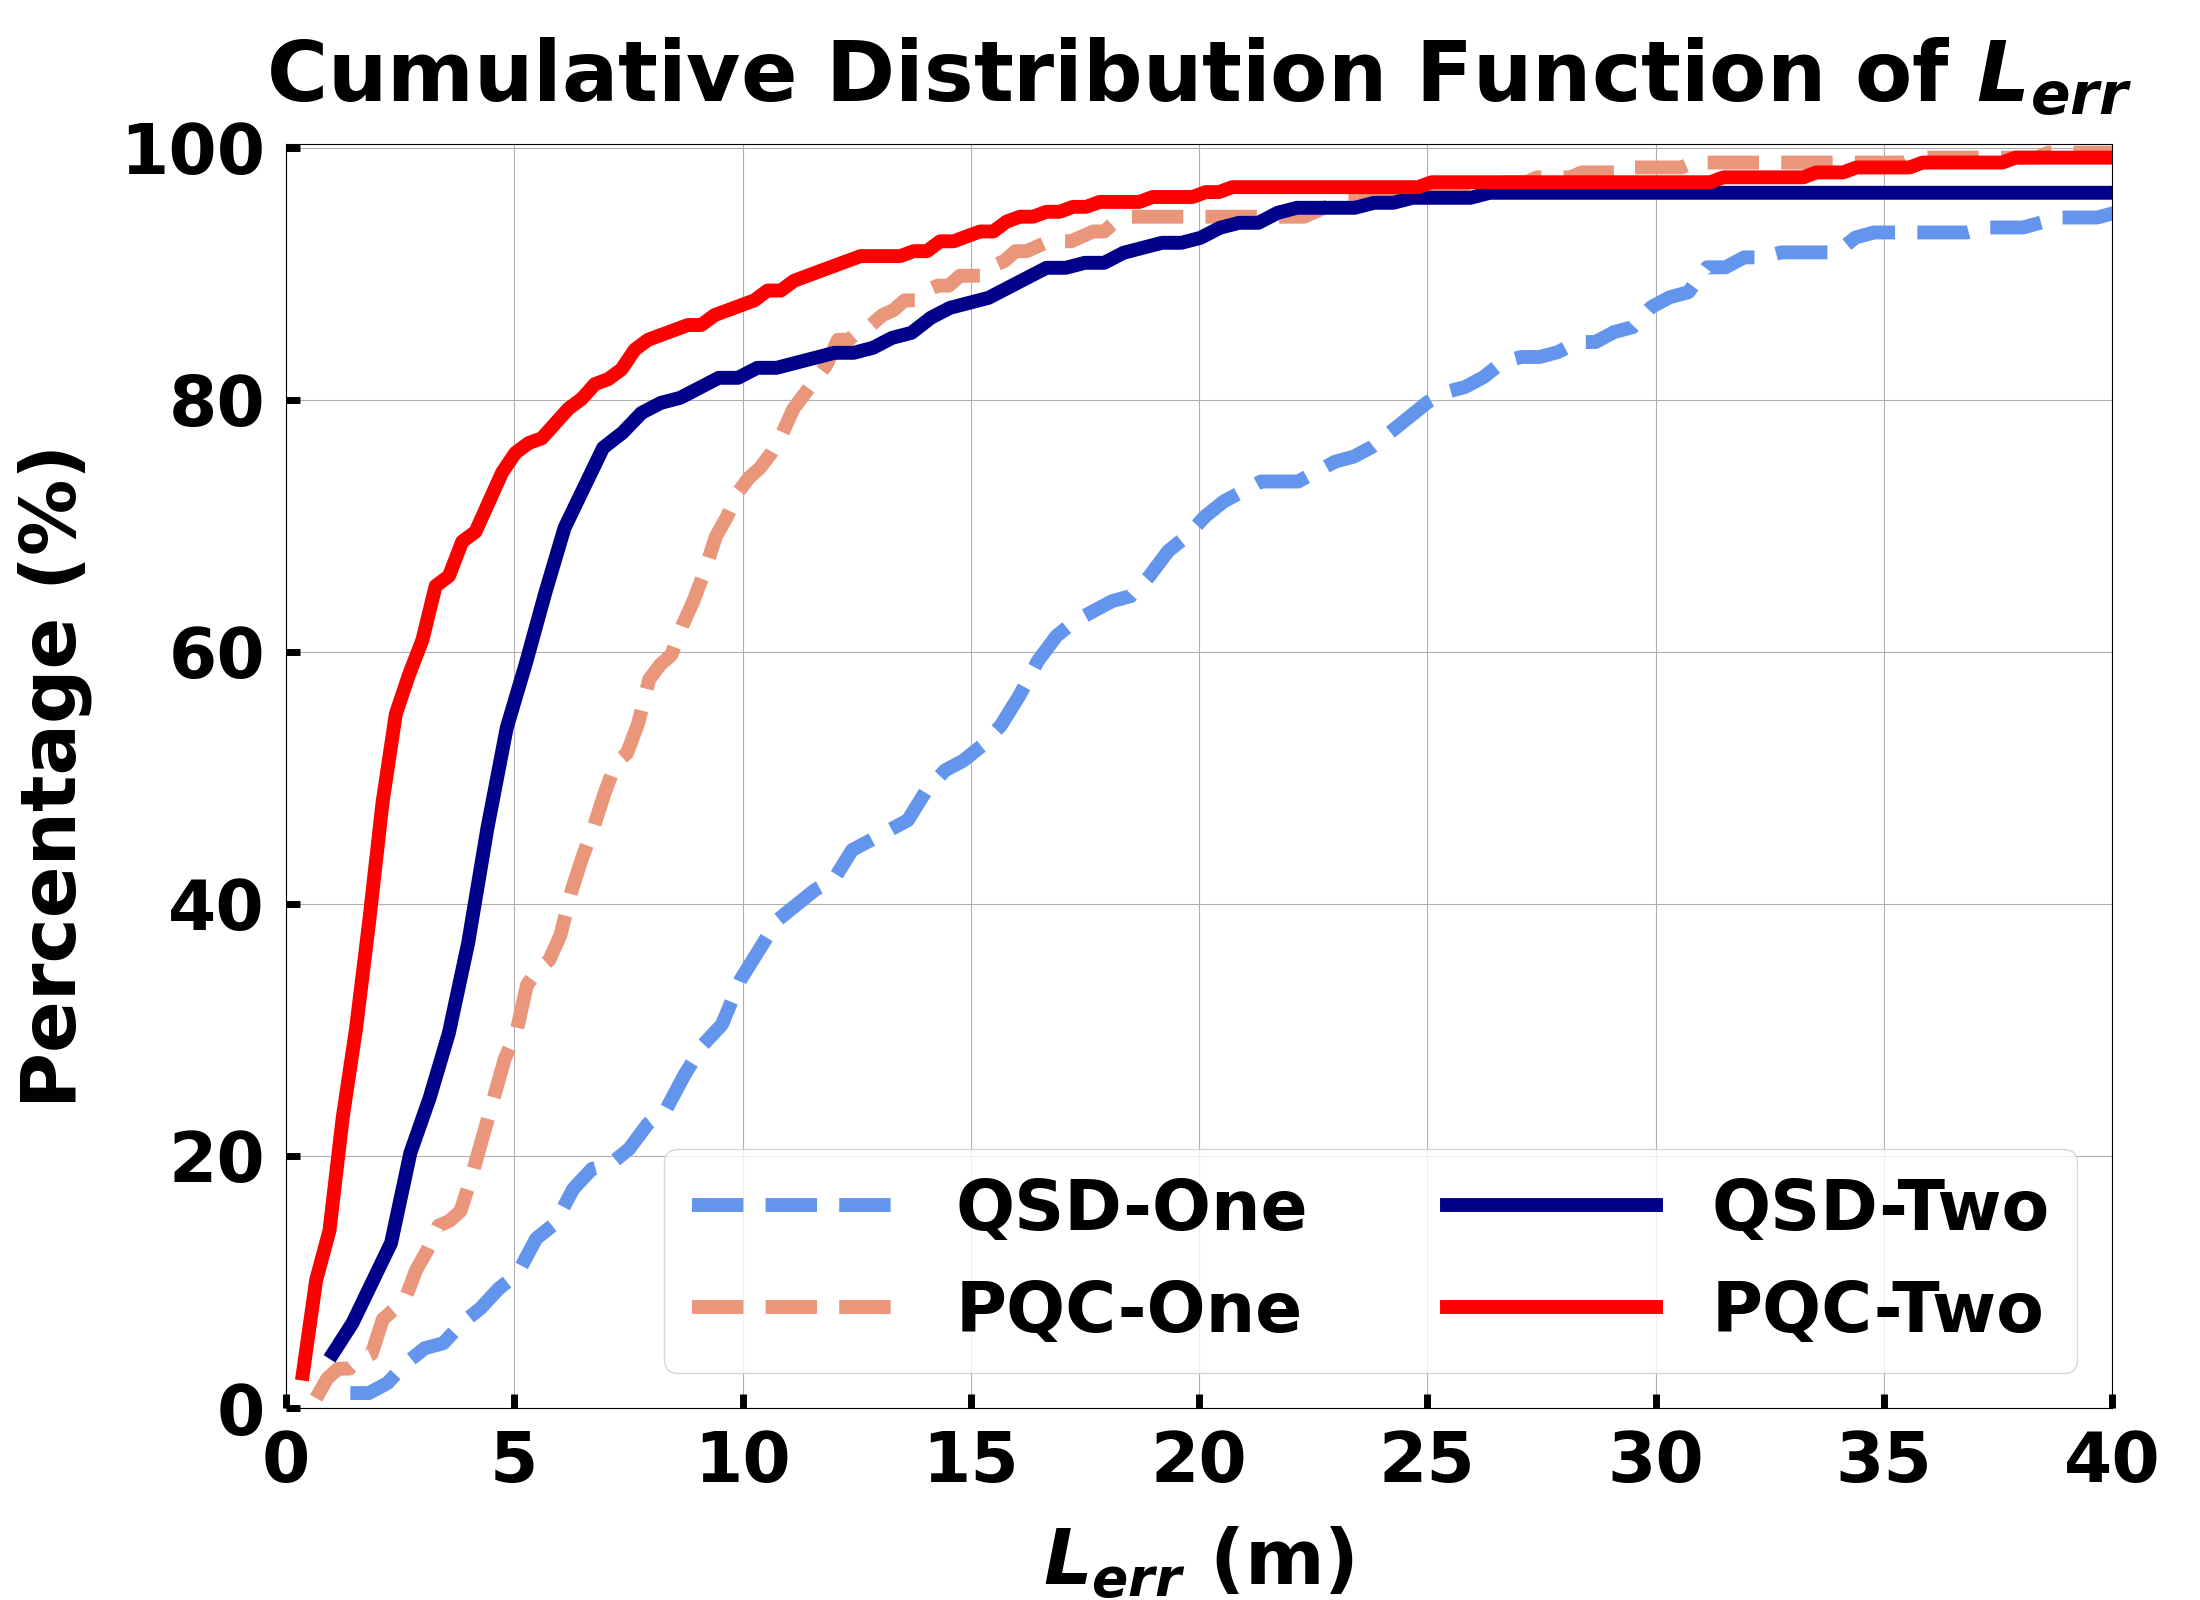
\includegraphics[width=0.8\textwidth]{chapters/qce/figures/error_cdf.png}
    \caption{The cumulative probability of $\lerr$ of \povmone, \povm, \pqcone, \pqctwo for a $16\times16$ grid and 8 quantum sensors.}
    \label{fig:continuous.errorcdf}
\end{figure}

\para{CDF.}
Fig.~\ref{fig:continuous.errorcdf} shows the cumulative distribution function of $\lerr$ for four methods when the grid size is $16\times16$ and the number of sensors is 8.
This plot gives insight into the {\em distribution} of $\lerr$ over different TX location, 
compared with Fig.~\ref{fig:continuous.varysen} which shows only average $\lerr$ across many TX locations. 
Here, the distribution is over 256 TX locations---one random TX location per cell for 256 cells in the $16\times 16$ grid.
%%%%%%%%%%%%%%%%%%%%%%%%%%%%%
We observe, as expected, that  the two-level schemes are better than the one-level schemes, and the PQC-based methods are better than the QSD-based methods, except that \povm has a better CDF plot than
\pqcone up to the 83-th percentile. The above exception implies that \povm has higher number of locations with large $\lerr$ compared with \pqcone;
this is likely due to \povm incurring errors in determining the block at the first/coarse level, which can lead to large localization errors.
% \sout{But in most cases, the performance of \povm is actually better than \pqcone.
% So the $95\%$ percentile performance of \povm is poor, making the overall average $\lerr$ worse than \pqcone.}

% \begin{figure}[h]
%     \centering
%     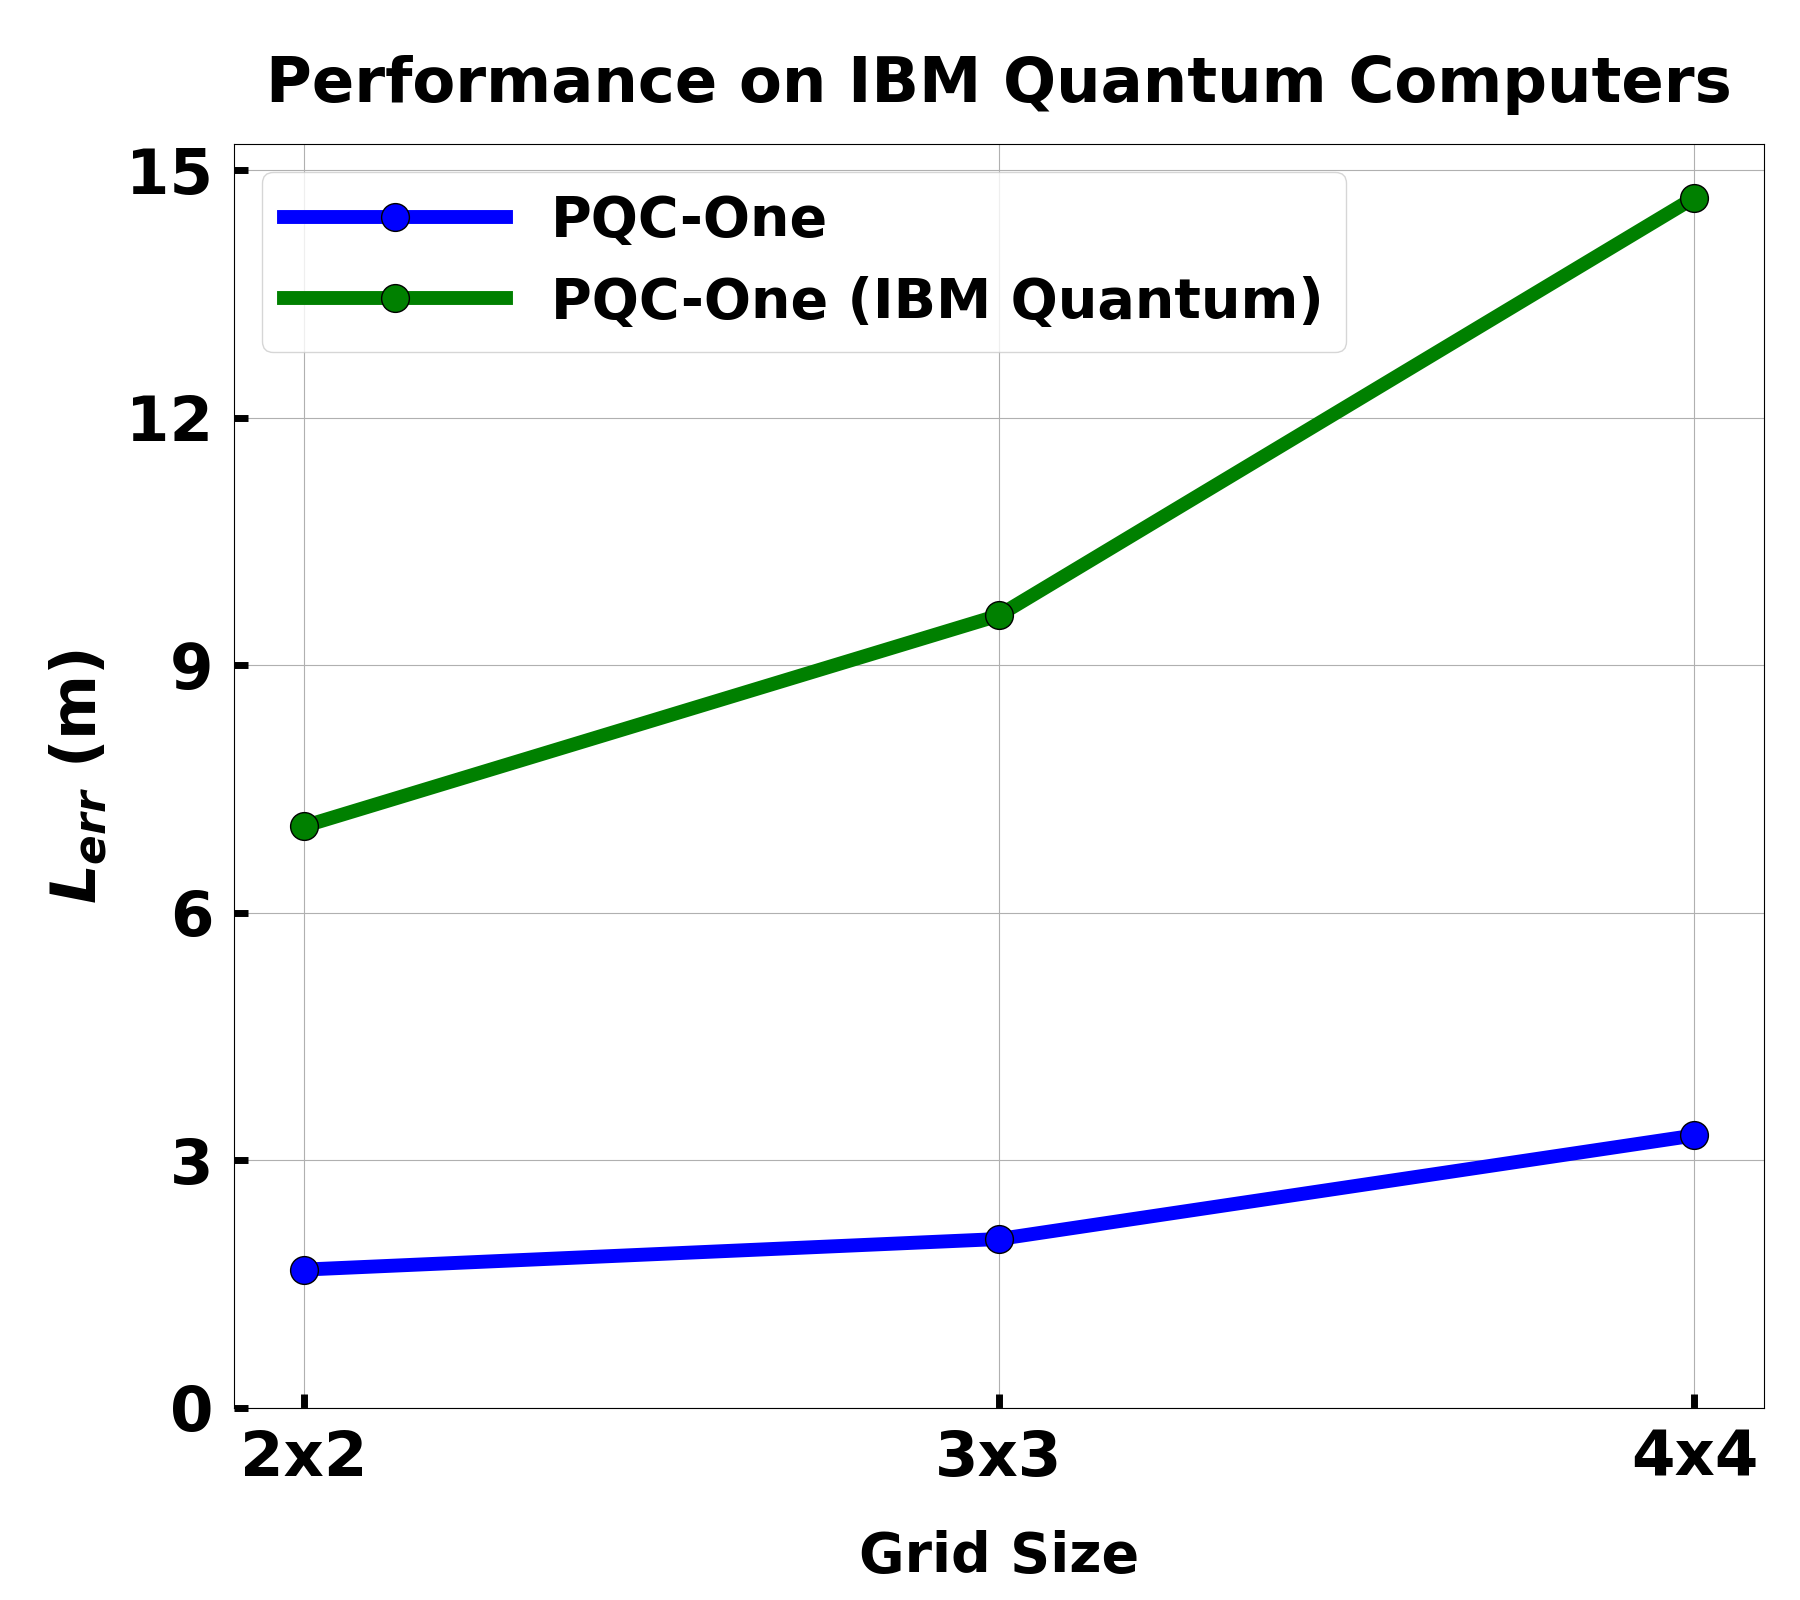
\includegraphics[width=0.32\textwidth]{figures/continuous.varygrid.ibm.png}
%     \caption{\red{ IBM quantum results}}
%     \label{fig:ibm-continuous-varygrid}
% \end{figure}


% \begin{figure}[h]
%     \centering
%     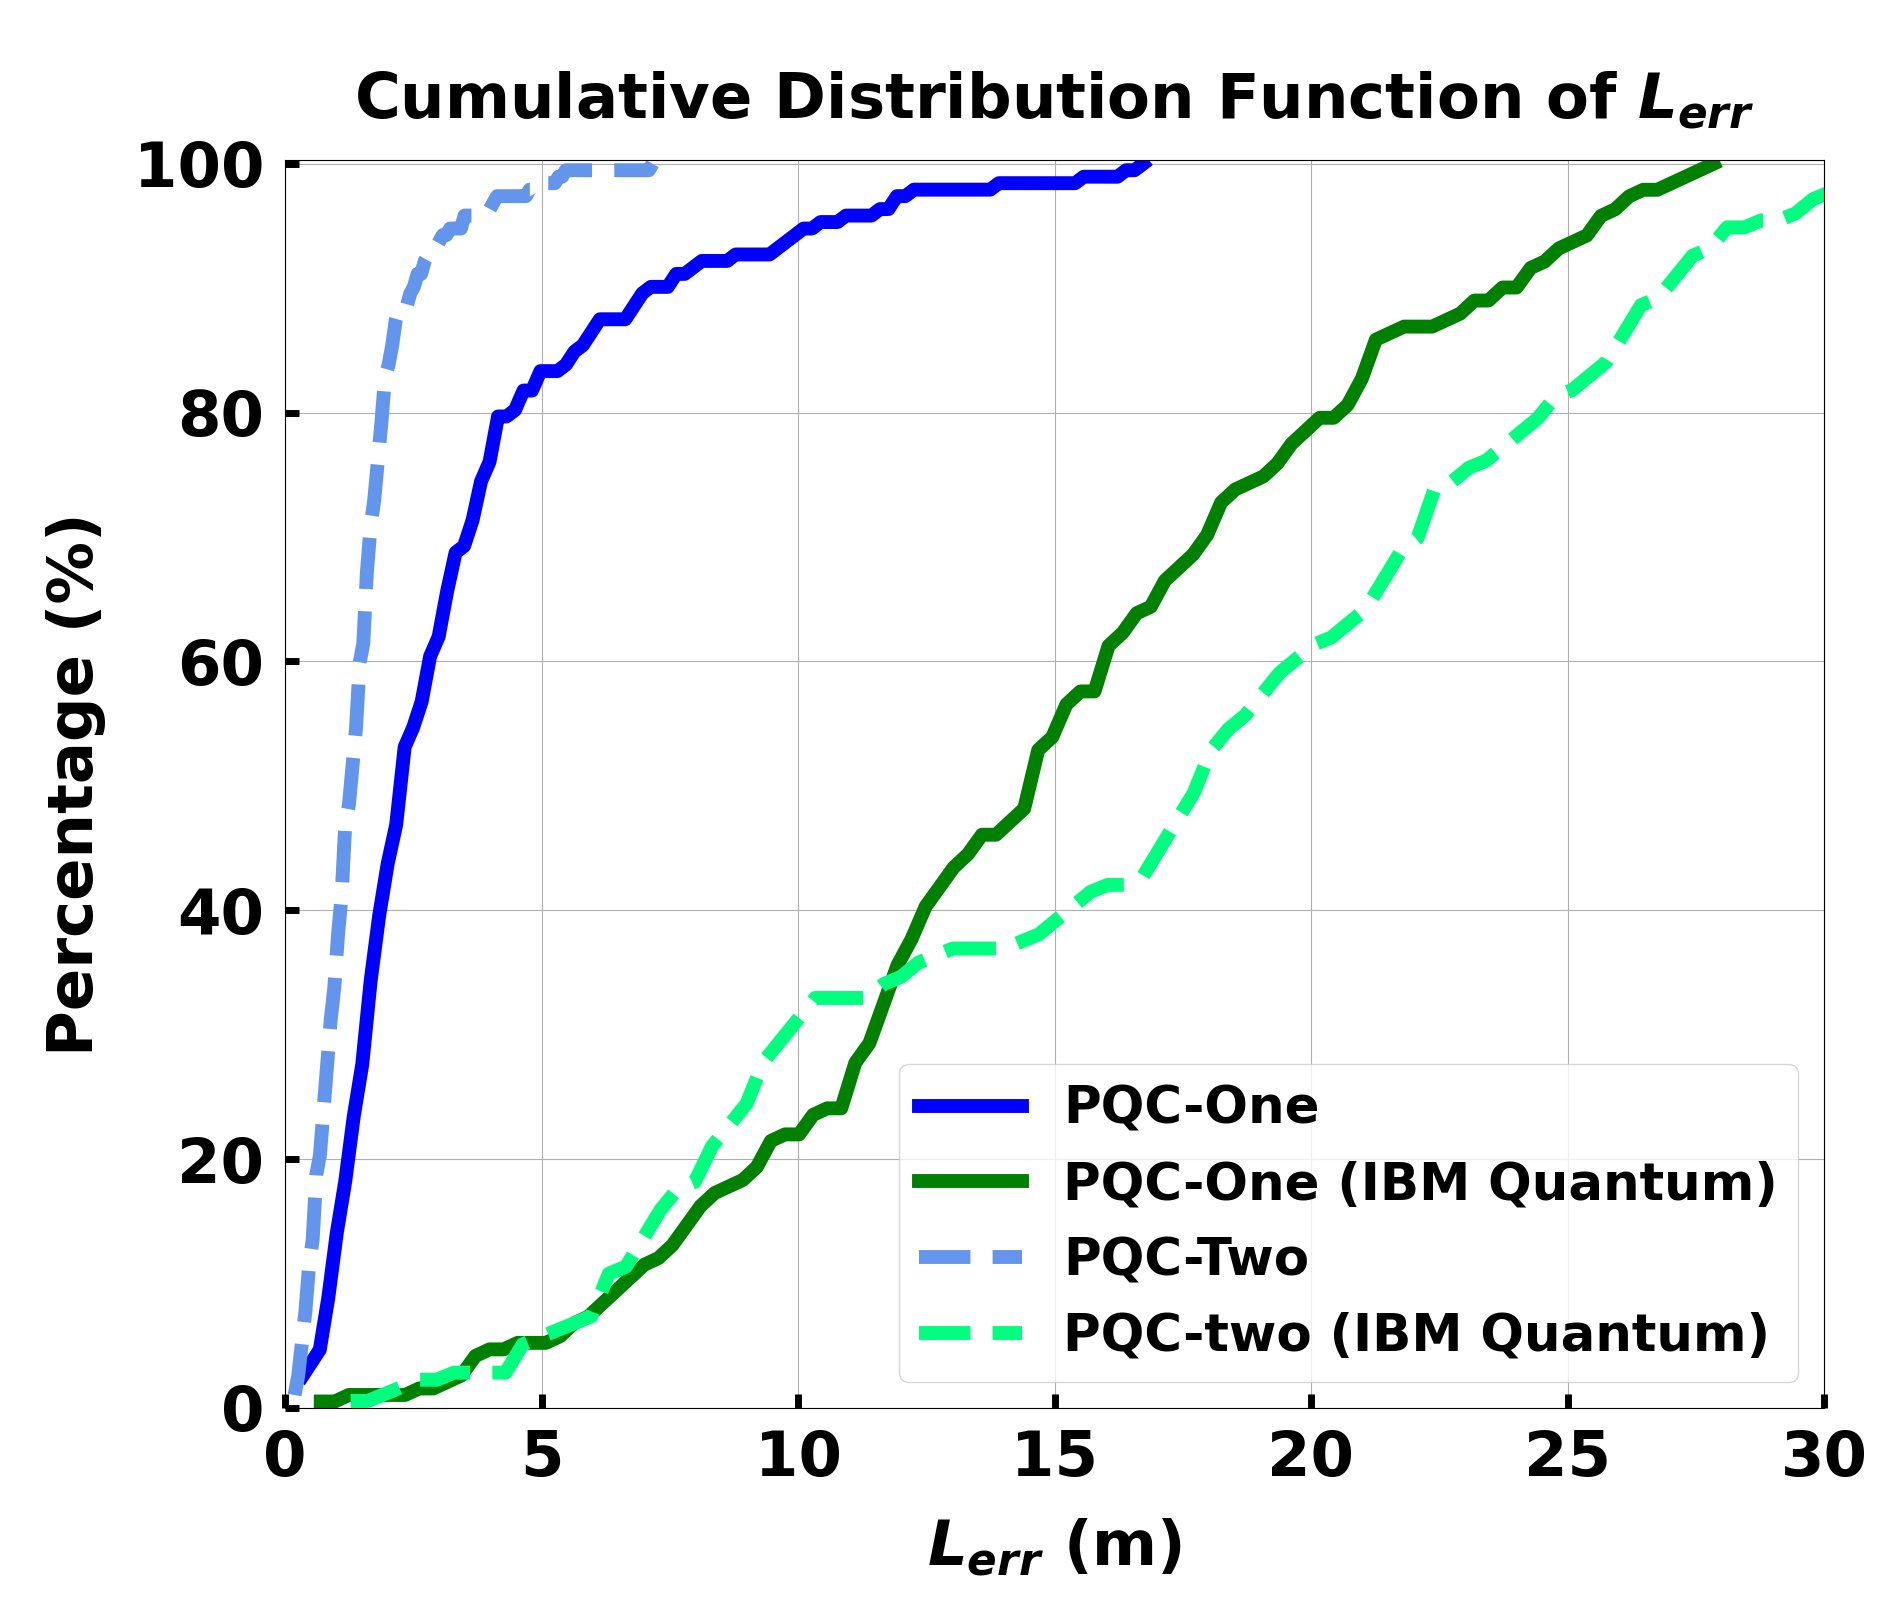
\includegraphics[width=0.32\textwidth]{figures/error_cdf_ibm.png}
%     \caption{\red{ IBM quantum results}}
%     \label{fig:ibm-continuous-cdf}
% \end{figure}


% \begin{figure}
% 	\centering
% 	\begin{subfigure}[t]{0.24\textwidth}
% 		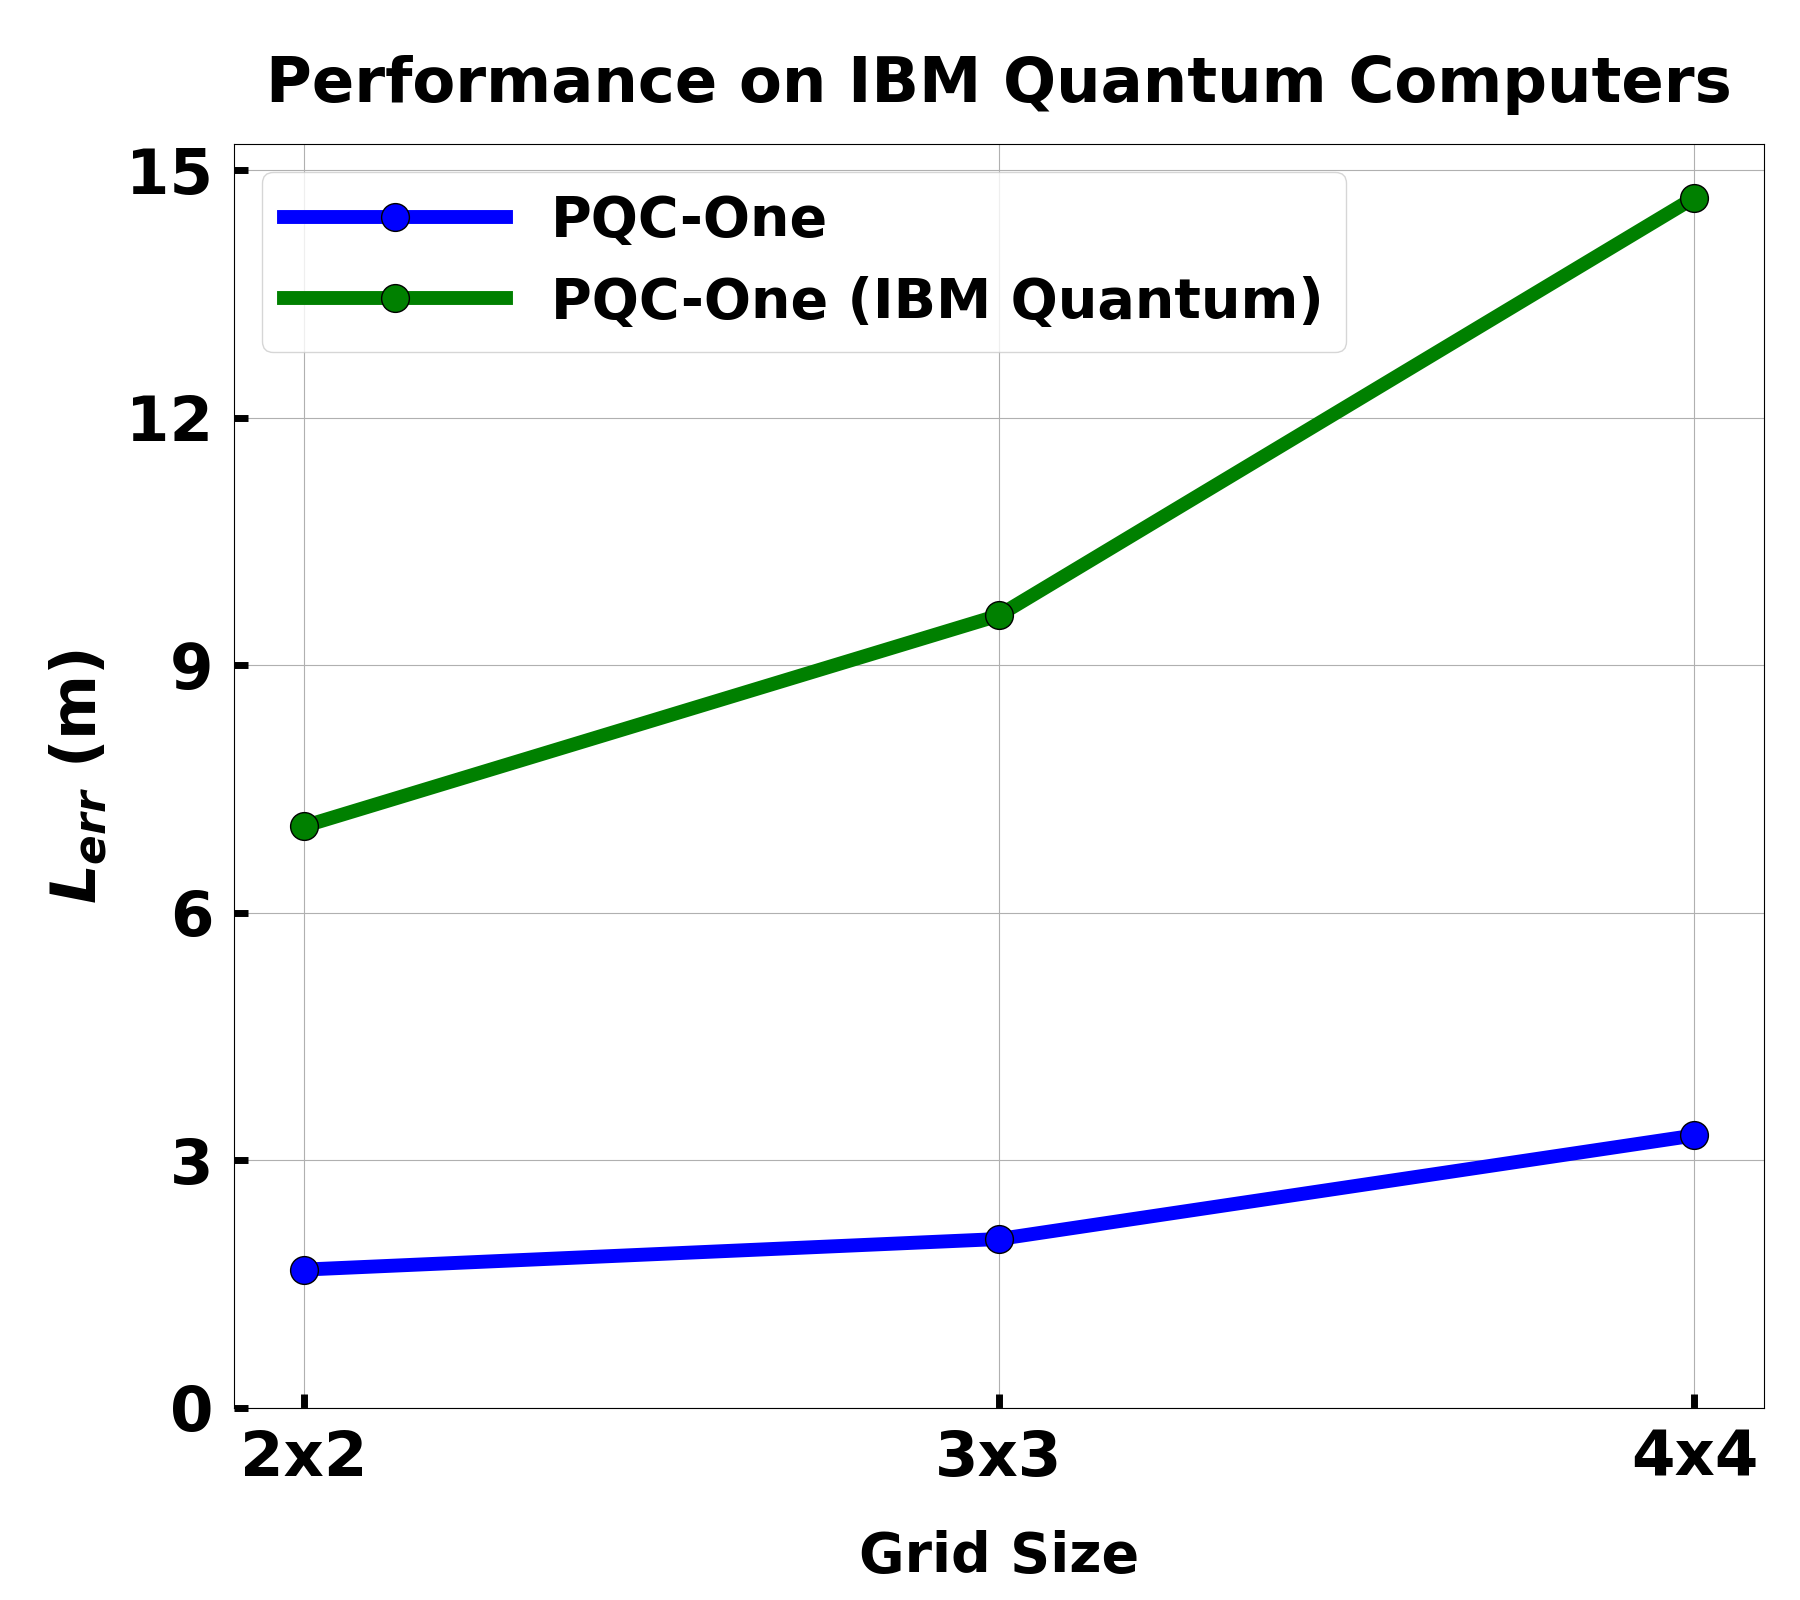
\includegraphics[width=\textwidth]{figures/continuous.varygrid.ibm.png}
% 		\caption{Varying grid size}
% 	\end{subfigure}
% 	\qquad
% 	\hspace{-0.4in}
% 	\begin{subfigure}[t]{0.24\textwidth}
% 		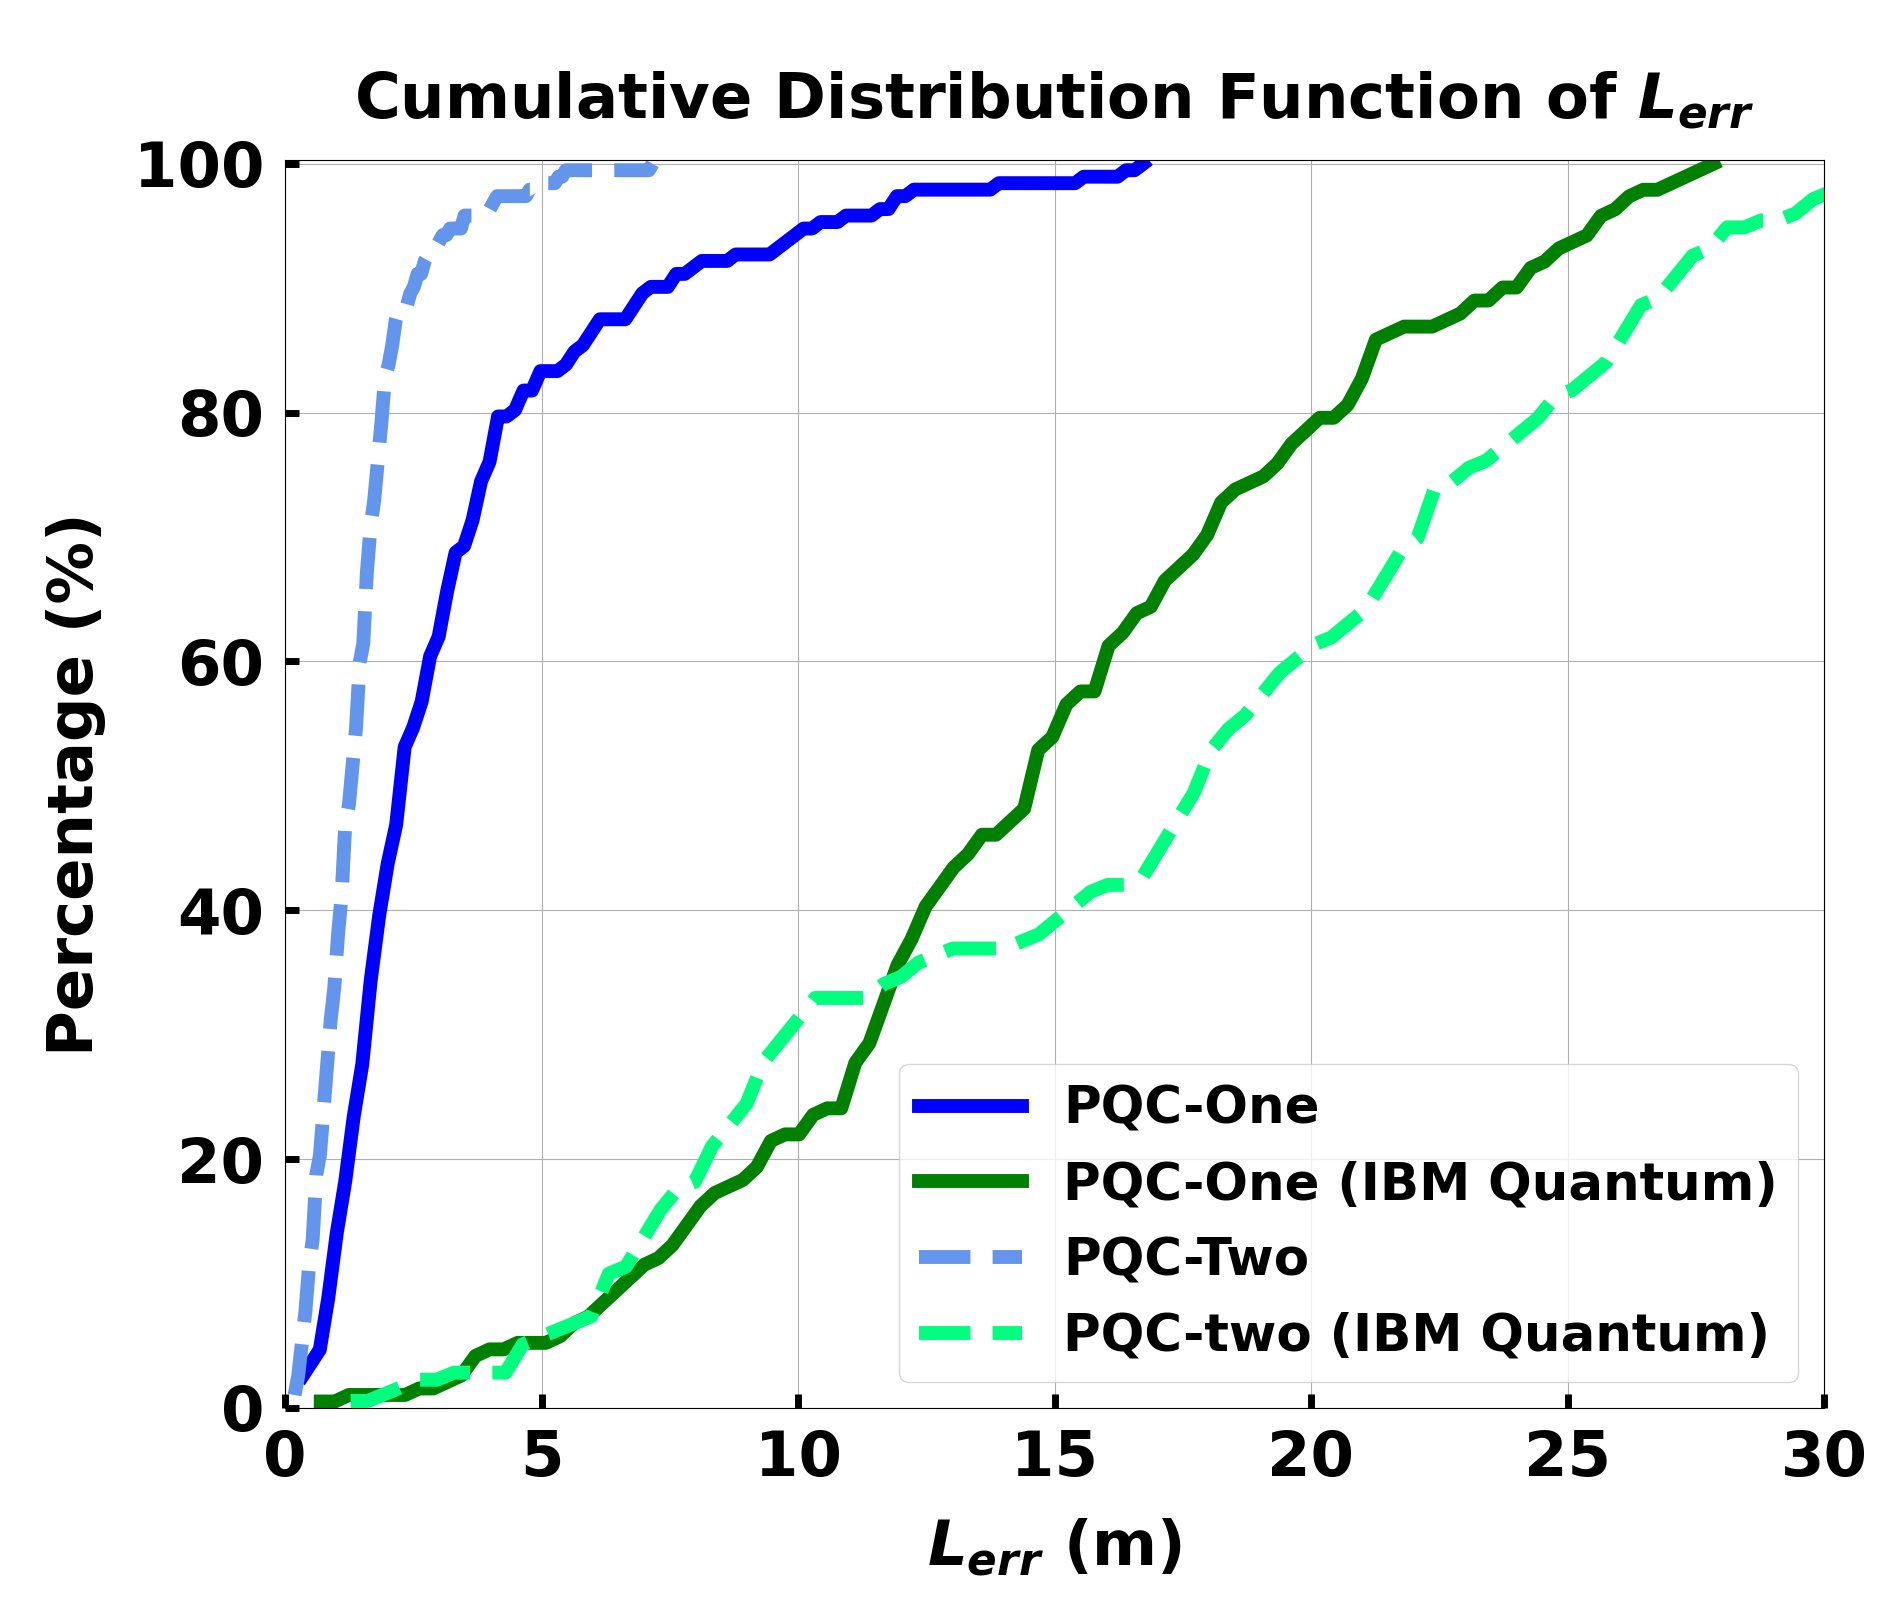
\includegraphics[width=\textwidth]{figures/error_cdf_ibm.png}
% 		\caption{One-level vs. two-level}
% 	\end{subfigure}
% 	\caption{Performance on IBM Quantum computer Manila.}
% 	\label{fig:ibm-continuous}
% \end{figure}


% \para{Incorporating Noise using IBM Quantum Computer.}
% Fig.~\ref{fig:ibm-continuous} shows the performance of the PQC-based methods under noise.
% Since our parameterized quantum circuits are implemented and trained in TrochQuantum, we convert our trained circuits into Qiskit~\cite{Qiskit}, so that we can run the quantum circuits on an IBM Quantum machine.

\para{Discrete Setting:} 
% \softpara{\povmone Performance.}
In the previous evaluation results, we have considered the practical {\em continuous} setting wherein the transmitter can be anywhere in the area.
%%%%%%%%%%%%%%%%%%%%%%
To evaluate the true performance of our QSD-based methods, which are fundamentally classification strategies, we now evaluate the discrete setting
wherein the transmitter is located only at the center of a cell and the 
predicted output of a localization method is the cell number of the transmitter.
%%%%%%%%%%%%%%%%%%%%%%%%%%
In this {\em discrete} setting, we evaluate the performance metric of {\em Classification Accuracy} $\lacc$ which is the percentage of times the method is correct in predicting the {\em cell} number. 
Also, in this discrete setting, the PQC-based methods use the Classification variant in the location predictor component, while the QSD-based methods remain the same.

Fig.~\ref{fig:discrete.varygrid} shows the performance of the four algorithms with varying grid sizes when the number of quantum sensors is eight. We observe similar trend for each algorithm as well as similar relative trends among the
algorithms as in the continuous setting. 
%%%%%%%%%%%%%%
We make two important observations: 
\begin{enumerate}
    \item First, in the QSD-based methods, the \povm is a significant improvement over \povmone (from 13\% to 77\% for grid side $16\times16$), which shows the effectiveness of our two-level approach.
    \item Second, for the largest grid size of $16\times16$, the $\lacc$ for QSD-based \povm is reasonable at 77\% but is further 
improved impressively by \pqctwo at 97\%; this shows the effectiveness of our PQC-based methods. The 3\% error here in \pqctwo is mainly due to the errors in the first level of determining the block.
\end{enumerate}
Also, we see that for lower grid sides, the \povm surprisingly performs worse than \povmone; the 
reason for this is similar to the continuous case that determining the blocks at the first level becomes more erroneous when the grid size is small.


\begin{figure}[ht]
    \centering
    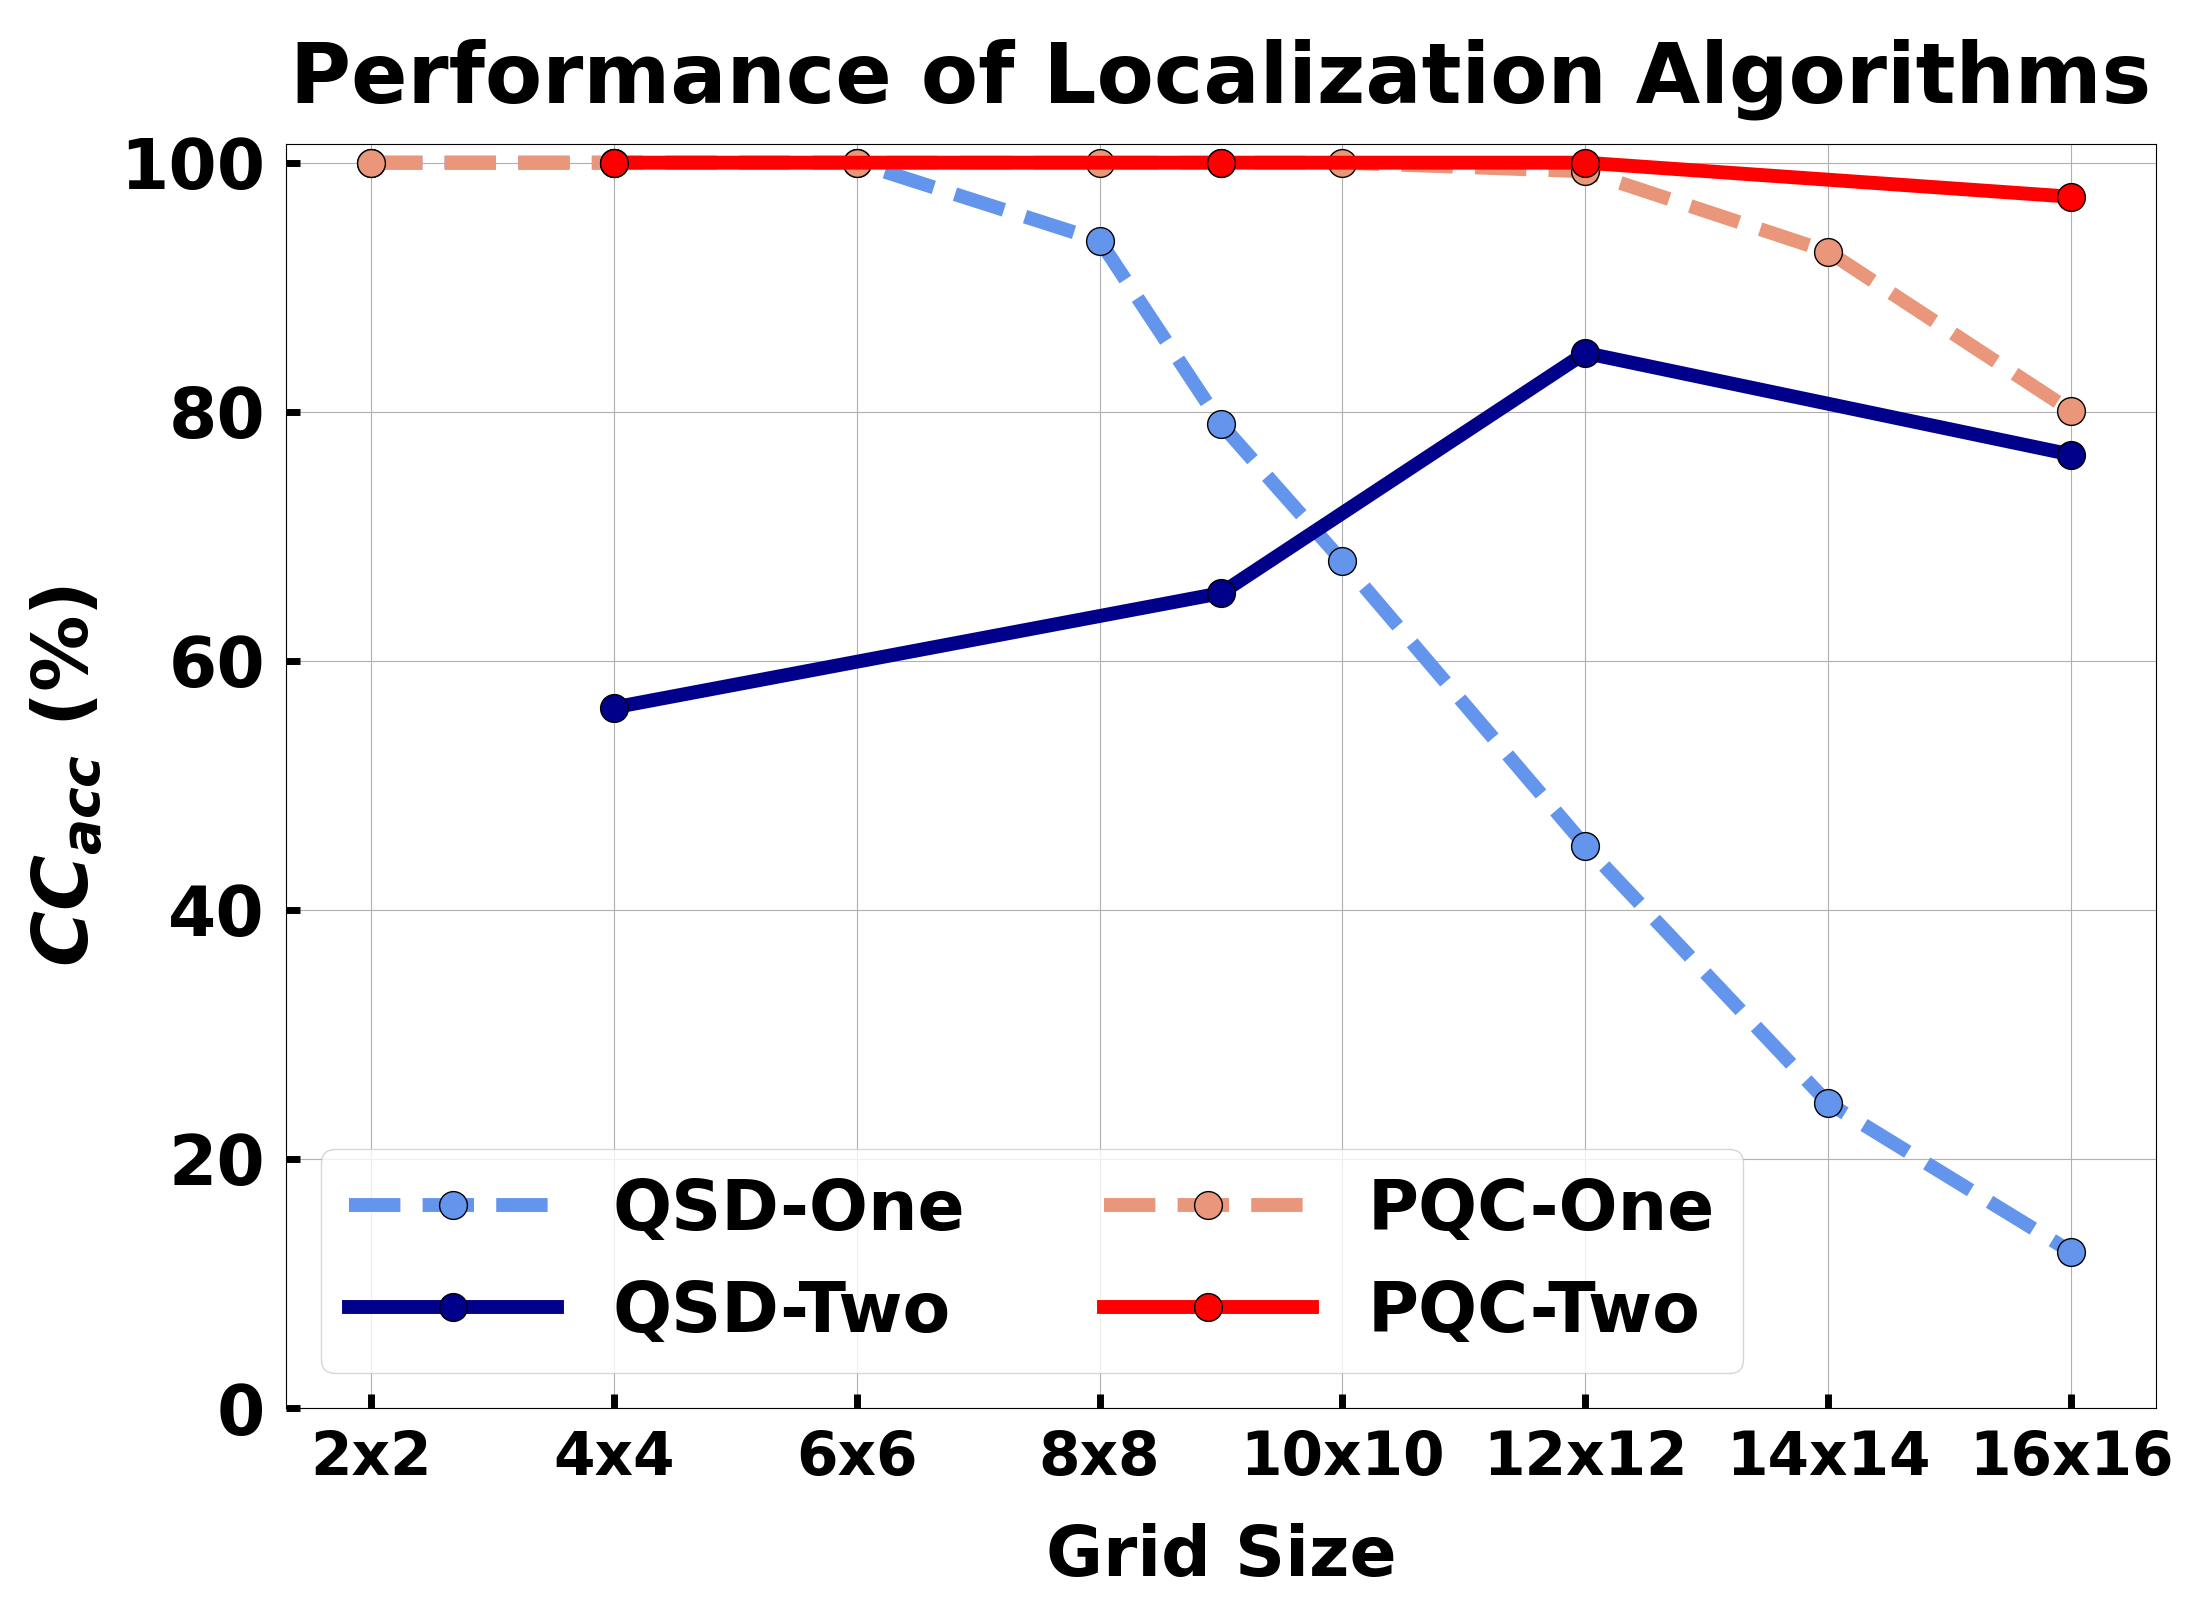
\includegraphics[width=0.8\textwidth]{chapters/qce/figures/discrete.varygrid.png}
    \caption{Performance of \povmone, \povm, \pqcone, \pqctwo for varying grid size and 8 sensors.}
    \label{fig:discrete.varygrid}
\end{figure}


\begin{figure}[ht]
    \centering
    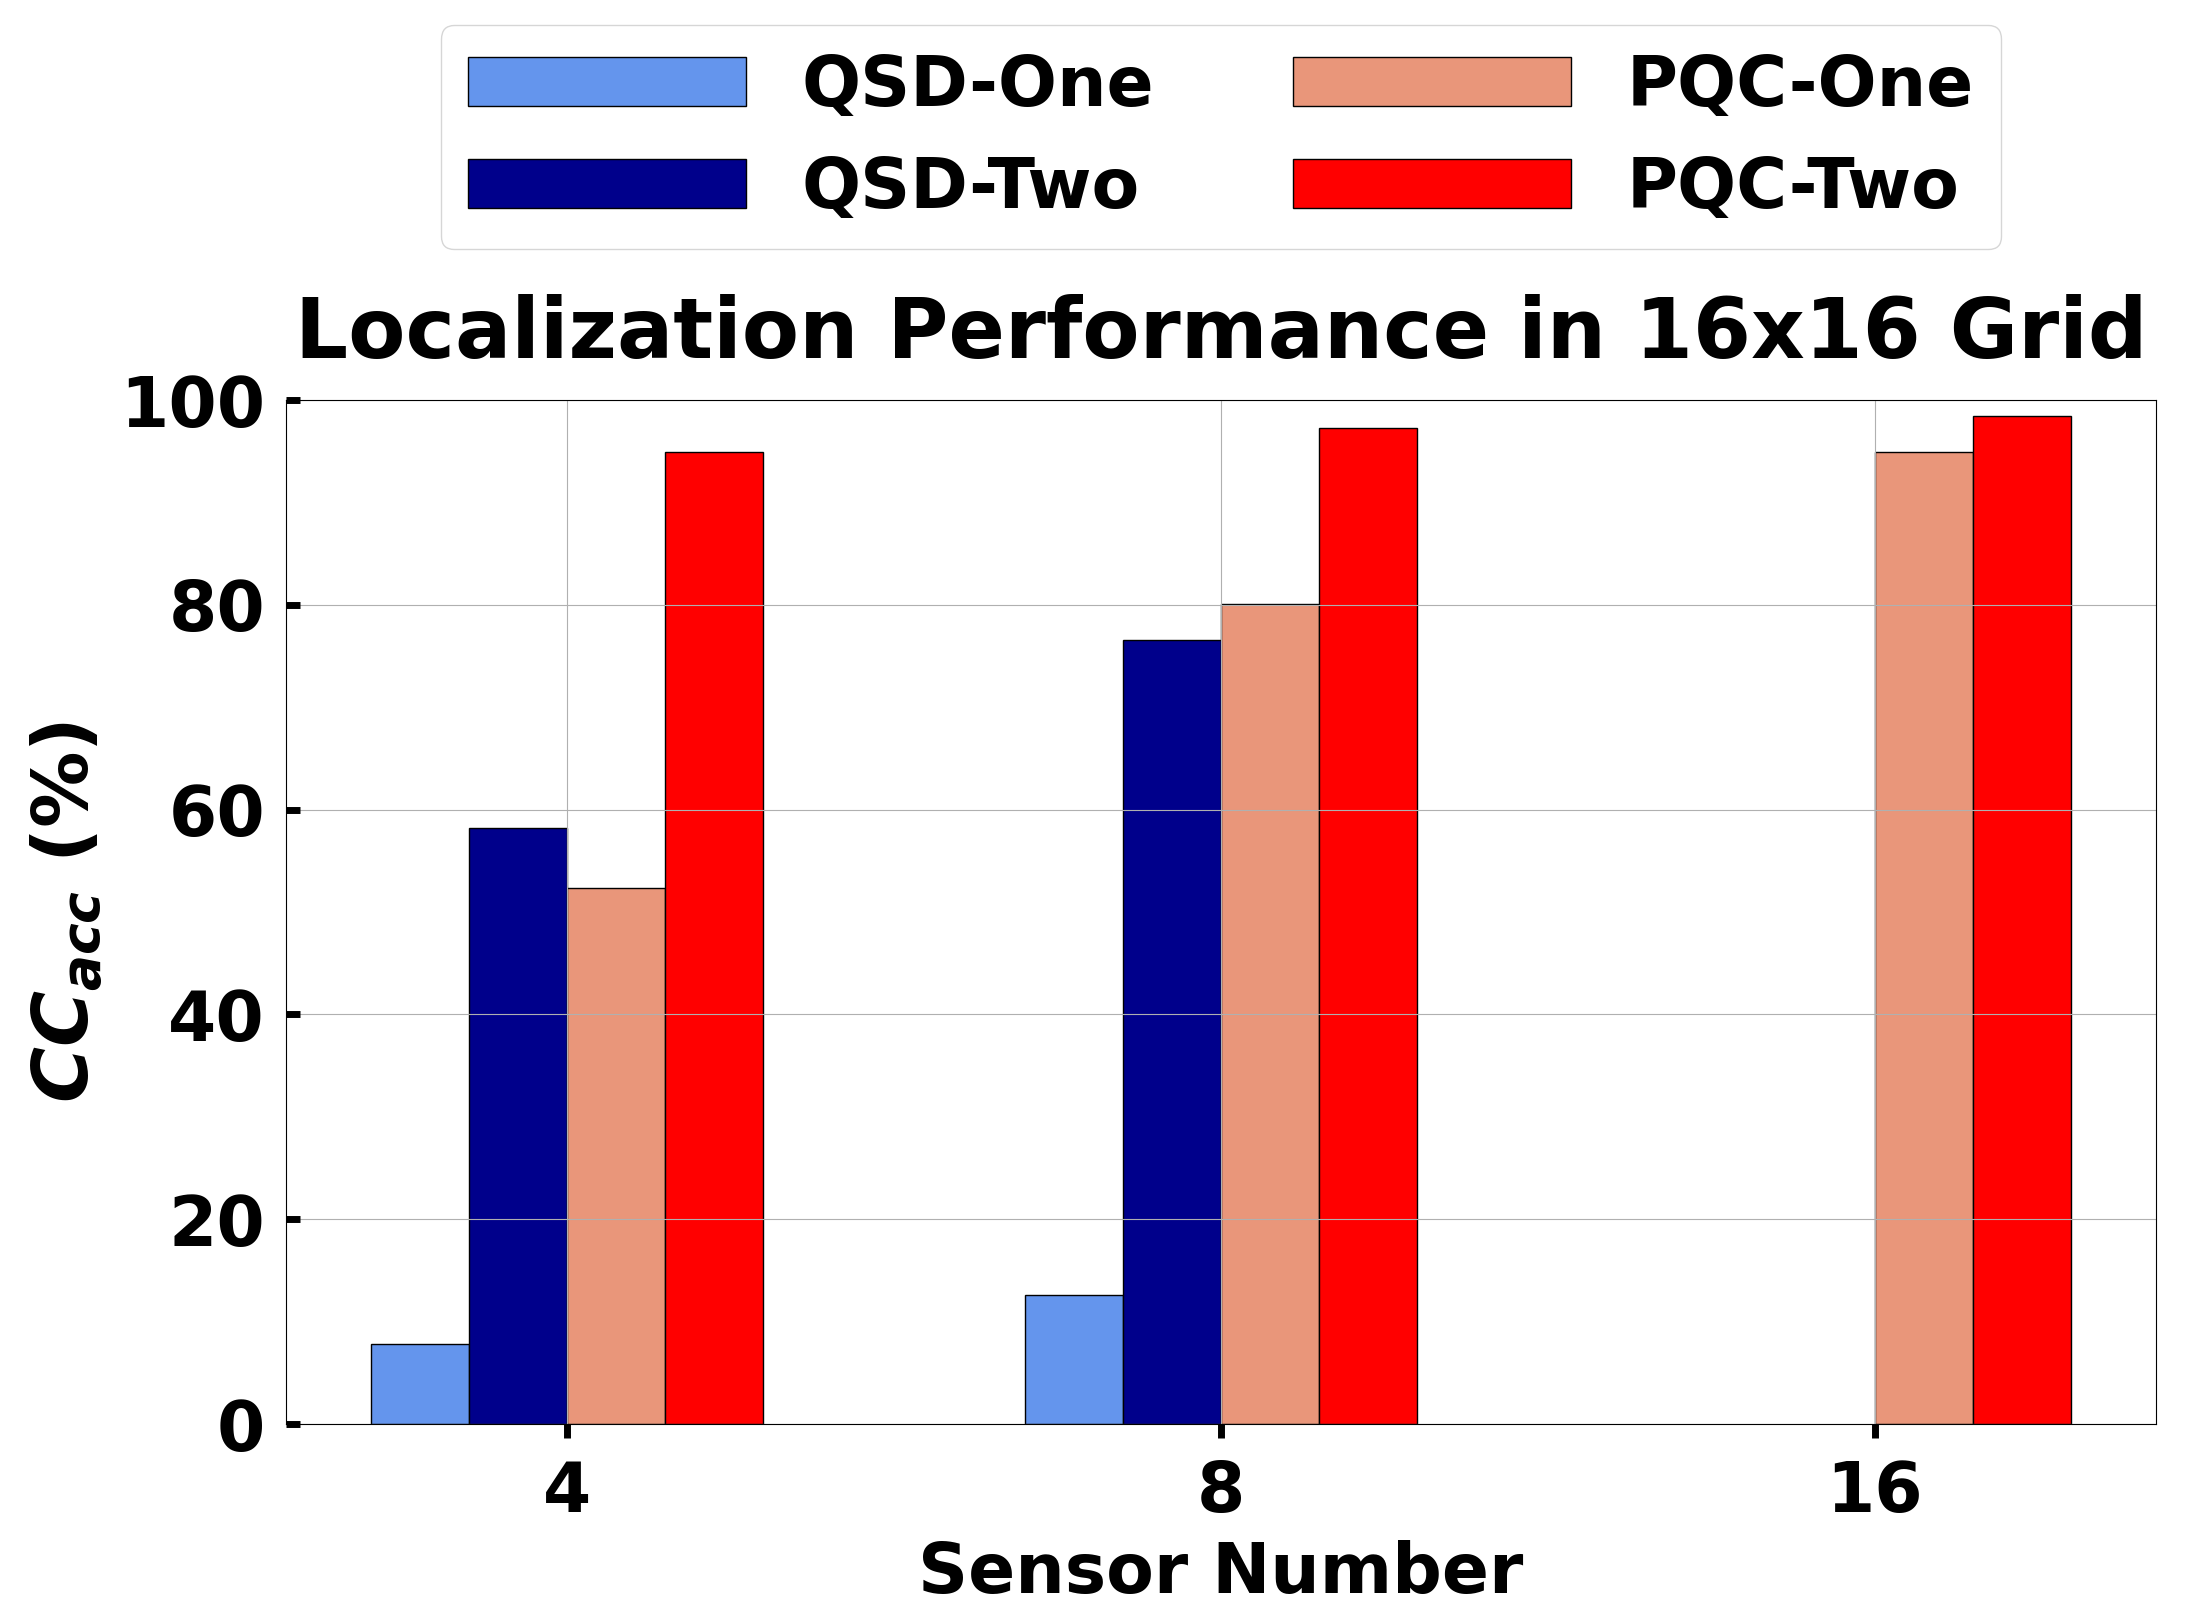
\includegraphics[width=0.8\textwidth]{chapters/qce/figures/discrete.varysensornum.png}
    \caption{Performance of \povmone, \povm, \pqcone, \pqctwo for varying sensor number and a $16\times16$ grid.}
    \label{fig:discrete.varysen}
\end{figure}


% \begin{figure}[h]
%     \centering
%     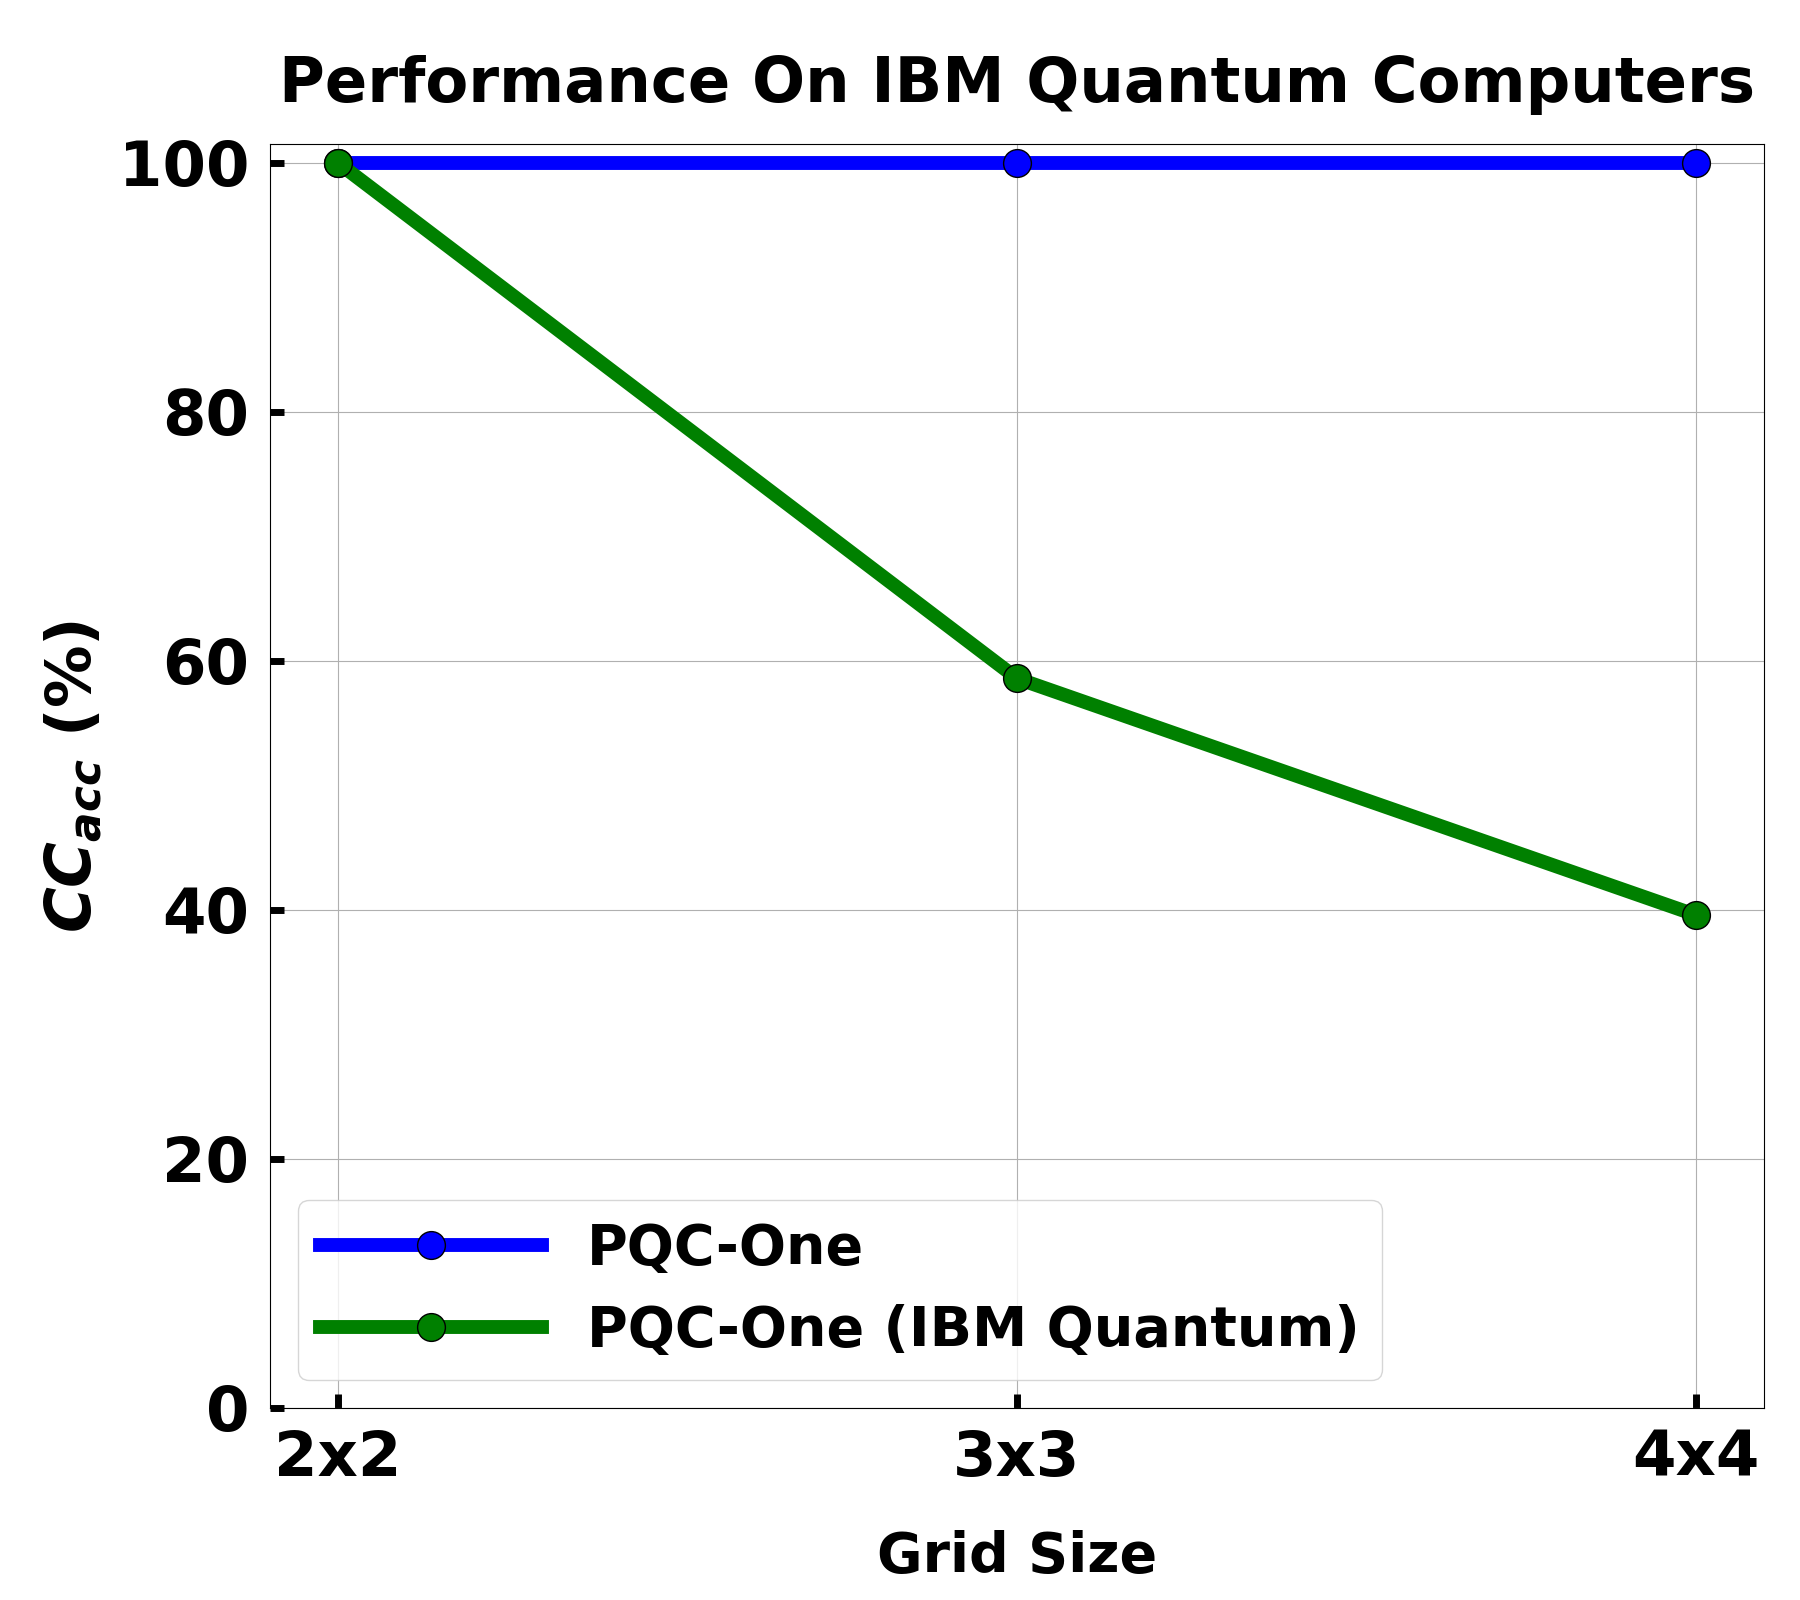
\includegraphics[width=0.32\textwidth]{figures/discrete.varygrid.ibm.png}
%     \caption{\red{ IBM quantum results}}
%     \label{fig:ibm-discrete-varygrid}
% \end{figure}

Fig.\ref{fig:discrete.varysen} shows the $\lacc$ in a $16\times16$ grid for varying number of quantum sensors. As expected, we observe that the $\lacc$ improves with an increasing number of quantum sensors. More importantly, the $\lacc$ for \pqctwo is {\em near-perfect} 
at $99\%$ with 16 sensors; this shows the effectiveness of the two-level method as well
as of the well-trained parameterized hybrid circuits. As in the continuous-domain setting, we don't show the QSD-methods for 16 sensors, as it was infeasible to implement the QSD-based methods for a large number of sensors.
